% Canonical entry point for Arithmetic Expression Geometry III.
\documentclass[11pt]{article}

\usepackage[letterpaper,margin=1in]{geometry}
\usepackage[T1]{fontenc}
\usepackage[utf8]{inputenc}
\usepackage[english]{babel}
\usepackage{lmodern}
\usepackage{amsmath,amssymb,amsthm,mathtools}
\usepackage{booktabs}
\usepackage{graphicx}
\usepackage{microtype}
\usepackage{xcolor}
\usepackage{tikz}
\usetikzlibrary{arrows.meta,positioning,calc,decorations.pathreplacing,decorations.markings}
\usepackage{url}
\usepackage[
  colorlinks=true,
  linkcolor=blue!45!black,
  citecolor=green!35!black,
  urlcolor=blue!55!black,
  pdfencoding=auto
]{hyperref}

\newtheorem{theorem}{Theorem}[section]
\newtheorem{proposition}[theorem]{Proposition}
\newtheorem{lemma}[theorem]{Lemma}
\newtheorem{corollary}[theorem]{Corollary}
\theoremstyle{definition}
\newtheorem{definition}[theorem]{Definition}
\newtheorem{example}[theorem]{Example}
\newtheorem{convention}[theorem]{Convention}
\theoremstyle{remark}
\newtheorem{remark}[theorem]{Remark}
\newtheorem{warning}[theorem]{Warning}
\newtheorem{problem}[theorem]{Open problem}

\newcommand{\R}{\mathbb{R}}
\newcommand{\C}{\mathbb{C}}
\newcommand{\F}{\mathbb{F}}
\newcommand{\Z}{\mathbb{Z}}
\newcommand{\Q}{\mathbb{Q}}
\newcommand{\HH}{\mathbb{H}}
\newcommand{\dd}{\,\mathrm{d}}
\newcommand{\AEG}{\mathrm{AEG}}
\newcommand{\Crit}{\operatorname{Crit}}
\newcommand{\Conf}{\operatorname{Conf}}
\newcommand{\UConf}{\operatorname{UConf}}
\newcommand{\ord}{\operatorname{ord}}
\newcommand{\Aff}{\operatorname{Aff}}
\newcommand{\id}{\operatorname{id}}
\newcommand{\pr}{\operatorname{pr}}
\newcommand{\im}{\operatorname{Im}}
\newcommand{\re}{\operatorname{Re}}
\newcommand{\calZ}{\mathcal Z}
\newcommand{\calR}{\mathcal R}
\newcommand{\calD}{\mathcal D}
\newcommand{\sfP}{\mathcal P^{\mathrm{sf}}}
\newcommand{\Spec}{\operatorname{Spec}}
\newcommand{\Gal}{\operatorname{Gal}}

\title{\textbf{Arithmetic Expression Geometry III:\\Singular Zero Geometry and Tubes}\\[0.45em]
\large Branched Pullbacks, Arithmetic Zero Networks, and Topological Transport}

\author{
Mingli Yuan\\
Swarma Research\\
Beijing 100083, China
}

\date{August 6, 2026\\[0.25em]
\small Mathematical-review manuscript}

\begin{document}
\maketitle

\begin{abstract}
Arithmetic expression geometry associates a real assignment to an oriented
Riemannian surface and imposes the eikonal identity
$|\nabla a|_g^2=\mu^2+\lambda^2a^2$, with $\mu\ne0$.  Its regular zeros are
curves, not isolated roots.  This paper develops the singular and parameterized
zero geometry needed to turn those curves into genuine tubes, while separating
them from the finite-root braids carried by complex-valued fields.

We first prove two complementary realization theorems.  Conformal rescaling makes
every surface submersion into a regular arithmetic expression space.  Holomorphic
branched pullback is more rigid: a local branch of degree $m$ produces a
$2m$-pronged singular zero and a metric cone of angle $2\pi m$.  The latter
mechanism yields an arithmetic global model.  The projective arithmetic operators
$z\mapsto z+\sqrt2$ and $z\mapsto-1/z$ generate the $(2,4,\infty)$ Hecke triangle
group.  From its normalized Hauptmodul we construct a singular AES whose zero set
is the Hecke dessin; after suppressing bivalent vertices it is the
$\{\infty,4\}$ zero network, with four-valent nodes and cone angle $4\pi$.

To separate arithmetic multiplicity from geometric branching, we introduce a
zero-history hierarchy and prove the standard relative-divisor decomposition for
a supplied monic generically square-free arithmetic polynomial.  Irreducible
factors over the
coefficient field, geometric sheets after scalar extension, and monodromy orbits
are distinct levels.  A functor assigning such a polynomial or divisor to a
general arithmetic history remains an open problem; the Hecke construction is
established at the projective-operator quotient level only.

A rank-$r$ parameterized zero-section theorem then gives the exact transversality
and properness hypotheses under which a zero incidence is a smooth fiber bundle.
For real assignments over a circle with globally oriented vertical tangent bundle,
every compact boundaryless proper zero tube is a union of tori.  An explicit
helical family computes component permutation, mapping-torus decomposition,
logarithmic deck shifts, and torus-link traces.

Topology change is confined to a discriminant.  Conformal Morse families realize
birth/death and reconnection in the singular category; the complex model
$w^2=\tau$ instead describes a branched filling whose boundary is a regular
half-twist.  Using the arithmetic-holomorphic coordinate of Paper II, every braid
is realized by a square-free polynomial root family.  Finally, affine conjugation
recovers an Alexander quandle.  Its ordinary torsion cocycle is exact, whereas a
finite-field resonant twisted version represents a nonzero twisted cohomology
class.  Nevertheless, we prove that its standard state sum for every planar
classical link collapses to the Alexander-quandle coloring count.  Thus it is not
evidence of a new invariant beyond Alexander or Burau.  Thread selection,
Markov-normalized AEG decorations, and any stronger separation theorem remain open.
\end{abstract}

\noindent\textbf{Keywords:}
arithmetic expression geometry; branched pullback; Hecke triangle group;
Hauptmodul; relative divisor; zero set; singularity; fiber bundle; braid group;
logarithmic covering

\setcounter{tocdepth}{2}
\tableofcontents
\newpage

\section{Singular AEG and the hierarchy of zero objects}
\label{sec:singular-aeg}
\subsection{The question}

Paper I associates to continuous affine evaluation a regular arithmetic expression
space
\[
  (M,g,a;\mu,\lambda),
  \qquad
  |\nabla a|_g^2=\mu^2+\lambda^2a^2,
  \qquad \mu\ne0,
  \tag{AEG}
  \label{eq:aeg-eikonal}
\]
where $M$ is an oriented smooth surface, $g$ is Riemannian, and $a$ is a
real-valued assignment function \cite{Yuan2026AEGFoundations}.  The right-hand
side of \eqref{eq:aeg-eikonal} is strictly positive.  Thus $a$ is a submersion,
and every nonempty level set---in particular $a^{-1}(0)$---is a regular curve.
An isolated zero, a crossing, a branch point, or a birth/death event cannot be a
regular interior zero.

The word \emph{tube} is nevertheless natural.  If an assignment varies with a
parameter, its zero curves sweep a surface in the product of the arithmetic
surface and the parameter space.  The central problem is to determine when that
swept surface is more than a picture: when it is smooth, when its projection is a
fiber bundle, where topology may change, and what additional data are needed
before a braid or knot can be extracted.

There is also a genuinely horizontal question.  Data already attached to one
slice do not by themselves relate two different slices.  A parameterized
polynomial can supply that relation: its imaginary part defines the moving real
carrier, while its full zero divisor defines a finite thread inside the carrier.
The family $z^2-t^m$ below makes this distinction explicit.  It is a supplied
relation rather than a general output of expression history, but its arithmetic
factorization, analytic discriminant period, carrier topology, and braid data can
be compared without changing the underlying object.

There is a second problem, logically prior to the tube: why should a complicated
zero set be attached to arithmetic expressions at all?  Conformal realization can
manufacture almost any regular zero pattern, so geometric abundance alone does not
answer this question.  The main analytic--arithmetic construction of this paper
starts instead from the projective operators of Paper I.  Translation by
$\sqrt2$ and negative inversion generate the $q=4$ Hecke group; its Hauptmodul
then produces a branched zero network whose four-valent vertices are forced by the
elliptic ramification.  This supplies an exact model in which arithmetic operator
paths, holomorphic branching, and singular AEG geometry meet.

The historical AEG notes used ``tube'' for several disjoint unions of ambient
geometries.  A source audit of the repository and its Git history found no
verifiable general construction under the old symbols $E_k$ or $E_{\log}$.
Accordingly, this paper does not import those symbols as established objects.
It constructs descriptive finite-zero, logarithmic-cover, and helical models from
first principles.  The distinction matters: an ambient family is not its zero
incidence, and a smooth zero incidence is not automatically a tube.

\subsection{Imported interfaces and new scope}

We use four results of Papers I and II as interfaces rather than redefining them.

\begin{enumerate}
\item Paper I proves the regular-zero theorem just recalled and defines a
  \emph{singular AES}.  Its singular set is closed, nowhere dense, and locally
  essential, and the regular equation holds on the complement.
\item Paper I proves that spatial regularity along the total zero set of a smooth
  real family makes that total zero set a smooth submanifold and its parameter
  projection a submersion.  It explicitly leaves global triviality open without
  properness.
\item Paper II equips every oriented regular AES with its underlying complex
  structure.  On the complete basic hyperbolic model, the arithmetic-holomorphic
  coordinate $w=X+iy$ is a global complex coordinate, and arithmetic
  holomorphicity is ordinary holomorphicity in $w$
  \cite{Yuan2026AEGFunctionTheory}.
\item Paper I's bilateral projective evaluation contains translations and negative
  inversion in $\operatorname{PGL}_2(K)$.  Over $K=\Q(\sqrt2)$ these operators
  generate the Hecke subgroup used in
  Section~\ref{sec:arithmetic-zero-networks}.  This import is at the operator
  quotient level and does not identify different raw history words or ordinary
  arithmetic domains \cite{Yuan2026AEGFoundations}.
\end{enumerate}

The first two interfaces concern a real scalar assignment and hence codimension-one
zero curves.  The third permits complex-valued auxiliary fields and hence
codimension-two isolated roots.  They must not be conflated.

\begin{definition}[Stratified singular AES]
\label{def:stratified-singular-aes}
A \emph{stratified singular AES} is a singular AES in the sense of Paper I together
with a specified locally finite Whitney stratification $\mathcal S$ of its singular
set $S$.  A stratum is called a \emph{singular zero stratum} if it is contained in
the closure of $a^{-1}(0)\cap(M\setminus S)$.  The stratification is additional
control data; it is not claimed to be canonical.
\end{definition}

This refinement supplies a language for parameterized Morse examples and branched
fillings.  It does not solve the classification of singular AEG germs.  Indeed, the
conformal realization theorem in Section~\ref{sec:local-zero-models} shows that the
bare singular-AES category is deliberately flexible.

\subsection{Seven levels that must remain distinct}

Let $q:X\to B$ be an ambient family and let $s$ be a real or vector-valued field on
$X$.  The following hierarchy fixes our terminology.

\begin{definition}[Zero-object hierarchy]
\label{def:zero-object-hierarchy}
Write $\calZ(s)=s^{-1}(0)$ and $\pi=q|_{\calZ(s)}$.
\begin{enumerate}
\item $\calZ(s)$ is the \emph{total zero set}; no regularity is implied.
\item It is a \emph{smooth zero incidence} if it is a smooth submanifold of $X$.
\item It is a \emph{proper zero tube} if $\pi$ is a surjective, proper smooth
  submersion (with the corresponding neat boundary hypotheses when boundaries are
  present).
\item It is an \emph{embedded zero tube} when its inclusion in the specified
  ambient family is retained as part of the data.
\item A \emph{threaded zero tube} is an embedded zero tube together with a specified
  finite multisection or other explicitly declared one-dimensional thread datum.
\item A \emph{braid closure} is obtained only after a finite moving-point system,
  an ambient surface, and a closure convention have been fixed.
\item A \emph{knot invariant} is a quantity on closures that has been proved
  independent of all presentation choices, in particular the appropriate
  conjugation and stabilization moves.
\end{enumerate}
\end{definition}

\begin{figure}[ht]
\centering
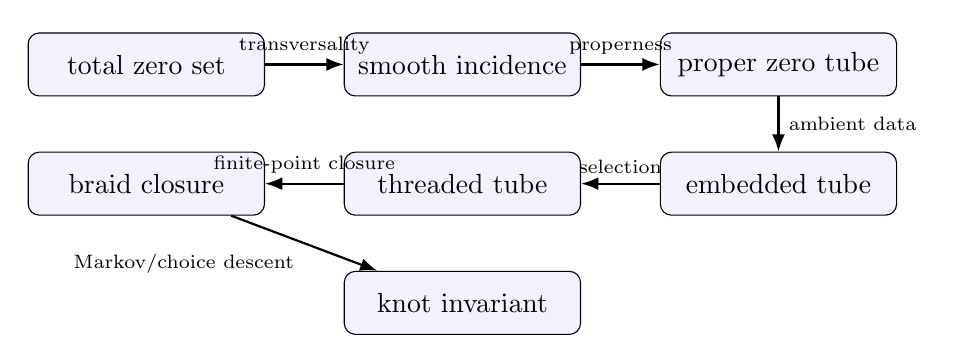
\begin{tikzpicture}[
  node distance=7mm and 10mm,
  box/.style={draw,rounded corners,align=center,minimum width=30mm,minimum height=8mm,
    fill=blue!5},
  arr/.style={-{Latex[length=2.2mm]},thick}
]
\node[box] (total) {total zero set};
\node[box,right=of total] (smooth) {smooth incidence};
\node[box,right=of smooth] (tube) {proper zero tube};
\node[box,below=of tube] (embed) {embedded tube};
\node[box,left=of embed] (thread) {threaded tube};
\node[box,left=of thread] (braid) {braid closure};
\node[box,below=of thread] (knot) {knot invariant};
\draw[arr] (total)--node[above,font=\scriptsize]{transversality}(smooth);
\draw[arr] (smooth)--node[above,font=\scriptsize]{properness}(tube);
\draw[arr] (tube)--node[right,font=\scriptsize]{ambient data}(embed);
\draw[arr] (embed)--node[above,font=\scriptsize]{selection}(thread);
\draw[arr] (thread)--node[above,font=\scriptsize]{finite-point closure}(braid);
\draw[arr] (braid)--node[below left,font=\scriptsize]{Markov/choice descent}(knot);
\end{tikzpicture}
\caption{Each arrow requires new hypotheses or data.  No arrow in the diagram is
automatic from the object to its left.}
\label{fig:zero-hierarchy}
\end{figure}

The hierarchy also exposes a dimension obstruction.  A real field on a surface has
one-dimensional zero fibers; a complex field has zero-dimensional root fibers.
Only the latter produces an ordinary geometric braid without an extra transverse
probe.

\subsection{Principal results}

The paper proves the following claims.  Status qualifications are included to make
the mathematical boundary visible.

\begin{table}[ht]
\centering
\small
\begin{tabular}{p{0.22\textwidth}p{0.50\textwidth}p{0.18\textwidth}}
\toprule
Result & Content & Status \\
\midrule
Conformal realization & Every smooth submersion on a surface satisfies
\eqref{eq:aeg-eikonal} for an explicit conformal metric. & Proved \\
Branched pullback & A holomorphic branch of degree $m$ gives a $2m$-pronged
essential zero and cone angle $2\pi m$. & Proved \\
Multi-zero models & Explicit regular AESs have exactly $k$ parallel zero
components, or countably many logarithmic lifts. & Proved \\
$q=4$ arithmetic network & A Hecke Hauptmodul gives the $\{\infty,4\}$ zero
network, $4\pi$ cone nodes, and sign-character descent. & Proved \\
Sign cover and cusp link & The completed coarse AEG surface of the sign cover is
$\C^\times$; retaining the hyperbolic orbifold, its unit tangent bundle is
$S^3\setminus T(2,4)$ under the standard cusp compactification. & Proved \\
Hecke geodesic knots & Primitive hyperbolic classes give periodic-orbit knots;
the zero dessin is their coding spine, and the cusp linking number is an explicit
turn sum using cited classical theorems. & Proved \\
Threaded carriers & The relation $z^2=t^m$ gives a genus-$(m-1)$
four-boundary carrier, $2m$ saddle events, thread $T(2,m)$, and one exact
discriminant--braid--Euler identity.  The $q=4$ marking also gives its toric and
logarithmic-tangent binomial forms and a supplied four-strand central
extension/transgression calibration. & Proved with data \\
Relative zero divisor & A supplied monic generically square-free arithmetic polynomial has
distinct $K$-prime, geometric-sheet, Galois, and monodromy levels. & Proved \\
Register naturality tests & Supplied quadratic and quartic registers give explicit
endpoint divisors, trace/pole data, collapse, discriminants, monodromy, and
Frobenius cycles. & Proved for supplied registers \\
General history divisor & A canonical functor sends unrestricted marked histories
to arithmetic prime relative divisors without losing required process data. & Open \\
Incidence theorem & Vertical transversality gives a smooth incidence and a
submersion; properness gives a bundle. & Proved with stated hypotheses \\
Real-tube structure & Compact boundaryless real zero tubes over $S^1$ with global
vertical orientation are unions of tori. & Proved with stated hypotheses \\
Helical tube & A compact family computes component permutation, logarithmic deck
shift, and torus-link boundary traces. & Proved \\
Singular models & Definite and indefinite Morse events satisfy the AEG equation
off an essential singular point. & Proved examples \\
Root monodromy & Square-free arithmetic-holomorphic polynomial families give
proper root coverings and realize every braid. & Proved via Paper II \\
Affine novelty filter & Stateless scalars collapse to writhe; ordinary affine
torsion is exact; resonant finite-field twisted torsion is nonzero but its planar
state sum collapses to coloring count. & Proved \\
Beyond baselines & A Markov-descended, choice-free AEG decoration separates
closures not separated by Alexander/Burau baselines. & Open \\
\bottomrule
\end{tabular}
\caption{Claim ledger for the main results.}
\label{tab:claim-ledger}
\end{table}

The positive and negative results are complementary.  The realization theorems
show that tube and braid geometry genuinely occur inside AEG.  The flexibility and
collapse theorems show that occurrence alone carries little discriminatory power.
Any new invariant must come from a natural decoration tied to expression history,
and that decoration must survive the relevant quotient.

\subsection{Organization}

Section~\ref{sec:local-zero-models} proves conformal and holomorphic pullback
realization, including finite Blaschke and essential-singularity controls.
Section~\ref{sec:multi-zero} records the flexible parallel and logarithmic models.
Section~\ref{sec:arithmetic-zero-networks} is the arithmetic core: it constructs
the $q=4$ Hecke--Hauptmodul singular AES, proves its character-valued descent, and
separates zero histories from relative prime divisors.
Section~\ref{sec:q4-geodesic-knots} identifies the sign cover, its cusp link,
and the precise coding-spine interface to Hecke periodic-orbit knots, without
identifying the two-dimensional zero graph with a three-dimensional template.
Section~\ref{sec:polynomial-threaded-carriers} uses one polynomial simultaneously
as a real carrier relation and a complex root thread, proves the horizontal
exact-sequence identities, and matches the marked $q=4$ cusp slopes.
Section~\ref{sec:history-divisor-naturality} tests divisor naturality on explicit
finite register covers and records the exact information lost at the operator
quotient.  Sections
\ref{sec:discriminants}--\ref{sec:singular-fibers} develop parameterized incidence,
proper tubes, and singular change.  Section~\ref{sec:braids} treats rank-two root
monodromy, and Section~\ref{sec:threading} applies the Markov and Alexander/Burau
novelty gates.  The logical order is therefore
\[
 \begin{gathered}
 \text{branched analytic germ}
 \longrightarrow\text{arithmetic zero network}\\
 \longrightarrow\text{relative divisor and discriminant}\\
 \longrightarrow\text{tube and monodromy}.
 \end{gathered}
\]

\subsection{Conventions}

All manifolds are smooth, Hausdorff, and second countable.  Unless boundary
hypotheses are stated, manifolds are boundaryless.  The parameters $\mu\ne0$ and
$\lambda\in\R$ always belong to the AEG equation; family parameters are denoted by
$b$, $t$, $\theta$, or $\tau$.  The letter $t$ is also used for an affine
multiplier only in Section~\ref{sec:threading}, where it cannot be confused with a
family coordinate.  A deck transformation is denoted $D$, while $T_{\mathrm{coef}}$
denotes the Laurent-module action in twisted quandle cohomology.

For a loop of configurations, a based loop determines a braid element and a free
loop determines a conjugacy class.  ``Invariant'' without qualification means an
ambient-isotopy invariant of oriented links; annular, transverse, framed, and
presentation-dependent data are named explicitly.


\section{Local zero models and conformal realization}
\label{sec:local-zero-models}
\subsection{The regular germ}

At a regular zero $p$, the submersion theorem gives coordinates $(u,v)$ centered
at $p$ in which $a=\mu u$: take $u=a/\mu$ and choose the sign of $v$ so that
$(u,v)$ is positively oriented.
This statement concerns the zero germ and the assignment; it does not put the
metric into Euclidean form.  Equation~\eqref{eq:aeg-eikonal} further gives
$|\nabla a|_g=|\mu|$ along $a=0$.  Thus a regular zero has one transverse
direction with a fixed nonzero speed and one tangent direction.  No finite-order
singularity can occur there.

The simplest global realization keeps the metric fixed.

\begin{example}[Cylindrical propagation]
\label{ex:cylindrical-propagation}
On $M=\R_r\times S^1_\phi$ with $g=\dd r^2+\dd\phi^2$, set
\[
 a_c(r,\phi)=
 \begin{cases}
  \dfrac{\mu}{\lambda}\sinh\!\bigl(\lambda(r-c)\bigr),&\lambda\ne0,\\[6pt]
  \mu(r-c),&\lambda=0.
 \end{cases}
\]
Then $|\nabla a_c|_g^2=\mu^2+\lambda^2a_c^2$ and
$Z(a_c)=\{c\}\times S^1$.  This model will yield a proper product tube in
Section~\ref{sec:regular-tubes}.
\end{example}

\subsection{Conformal realization}

The following construction is elementary, but it determines the scope of every
subsequent singularity claim.

\begin{theorem}[Conformal realization]
\label{thm:conformal-realization}
Let $(M,h)$ be an oriented Riemannian surface, let $a\in C^\infty(M,\R)$ be a
submersion, and fix $\mu\ne0$ and $\lambda\in\R$.  The conformal metric
\begin{equation}
 g_a=\frac{|\dd a|_h^2}{\mu^2+\lambda^2a^2}\,h
 \label{eq:conformal-realization-metric}
\end{equation}
is smooth and positive definite, and $(M,g_a,a;\mu,\lambda)$ is a regular AES.
\end{theorem}

\begin{proof}
Put $g_a=\rho h$.  Since $\dd a$ never vanishes and the denominator is positive,
$\rho$ is a positive smooth function.  The inverse metric is
$g_a^{-1}=\rho^{-1}h^{-1}$, so
\[
 |\nabla a|_{g_a}^2=|\dd a|_{g_a^{-1}}^2
 =\rho^{-1}|\dd a|_h^2
 =\mu^2+\lambda^2a^2.
\]
\end{proof}

\begin{corollary}[Singular realization]
\label{cor:singular-realization}
Let $a\in C^\infty(M,\R)$ have a closed nowhere-dense critical set
$S=\Crit(a)$.  On $M\setminus S$, define $g_a$ by
\eqref{eq:conformal-realization-metric}.  Then
$(M,S,g_a,a;\mu,\lambda)$ is a singular AES.  Every point of $S$ is locally
essential.
\end{corollary}

\begin{proof}
Theorem~\ref{thm:conformal-realization} applies on $M\setminus S$.  If a point
$p\in S$ admitted a regular local extension agreeing with $a$, then
$\dd a_p=0$ would imply $|\nabla a|^2(p)=0$ for the extended nondegenerate
metric, whereas the right-hand side of \eqref{eq:aeg-eikonal} is at least
$\mu^2>0$.  This is impossible.
\end{proof}

\begin{warning}[Flexibility boundary]
\label{warn:flexibility}
When the metric may be chosen as part of the construction, the regular AEG
equation admits every smooth submersion, and the singular category admits every
smooth function with closed nowhere-dense critical set.  Therefore the bare
equation does not by itself select an AEG-specific list of singularity types.
A classification theorem would require additional naturality or analytic
hypotheses, such as a fixed ambient metric, completeness, curvature bounds,
controlled metric asymptotics, homogeneity, or derivation from expression history.
\end{warning}

The warning is not a defect of the construction.  It is a precise division of
labor.  The equation controls assignment speed relative to a chosen metric; it
does not select that metric.  Later tube theorems are consequently topological
theorems with explicit hypotheses, not rigidity theorems for arbitrary AEGs.

\subsection{Singular zero mechanisms}

There are at least four mechanisms by which the regular-zero conclusion can fail.

\begin{enumerate}
\item The assignment may fail to be differentiable at a point, even though the
  metric extends there.
\item The assignment may be smooth but critical, forcing the conformal realization
  metric to degenerate or be removed at that point.
\item The domain may have a boundary or a puncture through which a zero component
  enters, exits, or escapes.
\item In a parameterized family, the total incidence may remain smooth while its
  projection to parameter space ceases to be a submersion.
\end{enumerate}

Paper I supplies a verified example of the first mechanism.  On the unit disc with
$\rho=(\xi^2+\eta^2)^{1/2}$, it takes
\begin{equation}
 g_{\mathbb D}=\frac{4}{\lambda^2(1-\rho^2)^2}
   (\dd\xi^2+\dd\eta^2),
 \qquad
 a_{\mathbb D}=\frac{2\mu}{\lambda}\frac{\rho}{1-\rho^2}
 \quad(\rho>0),
 \label{eq:imported-disc-model}
\end{equation}
with $a_{\mathbb D}(0)=0$ and $\mu,\lambda>0$.  The metric extends smoothly,
the assignment is not $C^1$ at the center, and the center is its only zero.  This
is an isolated singular zero, not a normal form for all isolated singular zeros.

The second and fourth mechanisms will appear together in the Morse families of
Section~\ref{sec:singular-fibers}.  The third is the reason properness and boundary
control occur explicitly in Definition~\ref{def:zero-object-hierarchy}.

\subsection{What local equivalence should preserve}

For clarity, we distinguish three notions that are sometimes compressed into the
phrase ``same singularity.''

\begin{definition}[Three local equivalences]
\label{def:three-local-equivalences}
For two pointed singular AEGs, a \emph{zero-germ equivalence} is a local
diffeomorphism carrying one zero germ to the other.  An \emph{assignment-germ
equivalence} additionally intertwines the assignments up to a local diffeomorphism
of the target fixing zero.  An \emph{AEG-germ isomorphism} preserves the assignment,
the oriented metric, and the constants $(\mu,\lambda)$.
\end{definition}

The real Morse lemma classifies assignment germs up to a much coarser right-left
equivalence.  Conformal realization then equips those germs with examples of AEG
metrics.  It does not show that all AEG-germ isomorphism classes are represented by
the displayed metrics, nor that the metric asymptotics are unique.

\begin{problem}[Rigidity beyond conformal realization]
\label{prob:singular-rigidity}
Find natural hypotheses derived from arithmetic evaluation under which the local
singular AEG germ has a finite classification, and determine which of the Morse and
branch models of Section~\ref{sec:singular-fibers} survive that restriction.
\end{problem}


\section{Multi-zero and logarithmic constructions}
\label{sec:multi-zero}
\subsection{A finite and locally finite construction}

The regular-zero theorem is local and does not limit the number of connected
components globally.  The next model gives a direct answer to the existence part
of the multi-zero problem.

\begin{theorem}[Parallel multi-zero model]
\label{thm:parallel-multi-zero}
Let $h\in C^\infty(\R)$ have only simple zeros.  On $M=\R^2$ define
\begin{equation}
 a_h(x,y)=e^x h(y)
 \label{eq:parallel-assignment}
\end{equation}
and
\begin{equation}
 g_h=
 \frac{e^{2x}\bigl(h(y)^2+h'(y)^2\bigr)}
      {\mu^2+\lambda^2e^{2x}h(y)^2}
 (\dd x^2+\dd y^2).
 \label{eq:parallel-metric}
\end{equation}
Then $(M,g_h,a_h;\mu,\lambda)$ is a regular AES and
\begin{equation}
 Z(a_h)=\coprod_{h(c)=0}\R\times\{c\}.
 \label{eq:parallel-zero-set}
\end{equation}
In particular, if
$h_k(y)=\prod_{j=1}^k(y-c_j)$ with distinct $c_j$, the zero set has exactly
$k$ connected components.
\end{theorem}

\begin{proof}
One has
\[
 \dd a_h=e^x h(y)\,\dd x+e^x h'(y)\,\dd y,
 \qquad
 |\dd a_h|^2_{\mathrm{eucl}}
 =e^{2x}\bigl(h^2+(h')^2\bigr).
\]
The simple-zero hypothesis implies that $h$ and $h'$ never vanish
simultaneously.  The coefficient in \eqref{eq:parallel-metric} is therefore smooth
and positive.  Theorem~\ref{thm:conformal-realization} proves the AEG identity,
and $e^x$ never vanishes, so \eqref{eq:parallel-zero-set} is immediate.
\end{proof}

\begin{remark}[What the index counts]
\label{rem:descriptive-index}
The polynomial example proves existence of a regular AES with $k$ zero components.
It does not prove uniqueness, completeness, homogeneity, or a canonical
classification by $k$.  We therefore call it the \emph{parallel $k$-zero model},
not $E_k$.  The old repository symbol $E_k$ had no stable definition: at different
times its subscript suggested construction order, zero count, or singularity count.
\end{remark}

Taking $h(y)=\sin y$ gives a countable, locally finite zero family.  This example
already suggests that countably many visible sheets may be repetitions under a
covering group rather than independent components of downstairs geometry.

\subsection{A downstairs model and its logarithmic pullback}

Let $z=X+iY$ be the standard coordinate on $\C^\times$ and set
\begin{equation}
 a_\times(z)=Y,
 \qquad
 g_\times=\frac{\dd X^2+\dd Y^2}{\mu^2+\lambda^2Y^2}.
 \label{eq:punctured-plane-aes}
\end{equation}
Since $|\dd Y|^2_{\mathrm{eucl}}=1$, this is a regular AES.  Its zero set is the
punctured real axis, hence has two components.

Pull \eqref{eq:punctured-plane-aes} back along the exponential covering
\[
 \exp:\C\longrightarrow\C^\times,
 \qquad x+iy\longmapsto e^{x+iy}.
\]
The resulting data are
\begin{equation}
 \widetilde a(x,y)=e^x\sin y,
 \qquad
 \widetilde g=
 \frac{e^{2x}}
      {\mu^2+\lambda^2e^{2x}\sin^2y}
 (\dd x^2+\dd y^2),
 \label{eq:logarithmic-aes}
\end{equation}
and
\begin{equation}
 Z(\widetilde a)=\coprod_{k\in\Z}\{y=k\pi\}.
 \label{eq:logarithmic-zero-lines}
\end{equation}

\begin{theorem}[Logarithmic zero lift]
\label{thm:logarithmic-zero-lift}
The data in \eqref{eq:logarithmic-aes} form a regular AES and are invariant under
the deck transformation
\[
 D(x,y)=(x,y+2\pi).
\]
On the labels in \eqref{eq:logarithmic-zero-lines}, $D$ acts by $k\mapsto k+2$.
Thus the countable upstairs zero family has exactly two deck orbits, corresponding
to the positive and negative real half-axes downstairs.
\end{theorem}

\begin{proof}
The formula is the pullback of the regular AES
\eqref{eq:punctured-plane-aes}; it can also be checked directly from
$|\dd\widetilde a|^2_{\mathrm{eucl}}=e^{2x}$.  Both $\sin y$ and the metric
coefficient are $2\pi$-periodic.  Finally,
$D(\{y=k\pi\})=\{y=(k+2)\pi\}$, proving the orbit statement.
\end{proof}

\begin{remark}[No singular spine at the missing origin]
The coordinate $z=0$ is absent from $\C^\times$, but the formula
$a_\times=Y$ and its metric extend regularly across it.  Hence the origin is not a
locally essential singularity in the sense of Paper I.  The model is a
\emph{logarithmic-domain model}, not an essential-singularity model.  Calling the
missing point a singular spine would erase the local-essentiality condition.
\end{remark}

Theorem~\ref{thm:logarithmic-zero-lift} is the rigorous content we retain from the
historical $E_{\log}$ intuition:
\[
 \text{countably many sheets upstairs}
 \quad=\quad
 \text{finite downstairs geometry plus deck labels}.
\]
No claim is made that it reconstructs every meaning previously attached to
$E_{\log}$.

\subsection{Sheet labels are not automatically topological states}

The label $k\in\Z$ in \eqref{eq:logarithmic-zero-lines} depends on a choice of
fundamental domain.  Its parity is invariant under the deck group in this model,
but an absolute integer label is not downstairs data.  More generally, logarithms
of moving complex roots acquire integer shifts whose individual values depend on
the chosen lifts; only cycle sums survive the lift gauge.  This statement is proved
in Section~\ref{sec:braids} and Appendix~\ref{app:configuration}.

There is a second obstruction to interpreting the parallel model as a braid.  If
$c_1(t)<\cdots<c_k(t)$ are distinct real zero positions throughout a one-parameter
family, their order cannot change without a collision.  The configuration space of
$k$ unordered points on a line has contractible components; it does not carry the
Artin braid group.  Noncommutative braid monodromy requires motion in a surface,
which in this paper comes from complex-valued fields, or else a separately declared
transverse probe.

\subsection{Metric completeness and provenance limits}

The models above are exact solutions of the AEG equation, but completeness is not
part of their claim.  For example, in the parallel model the conformal factor often
decays like $e^{2x}$ as $x\to-\infty$, placing that end at finite metric distance.
Completion can add boundary or singular strata and must be audited separately.
This is one reason the model record must always list the domain and metric, not only
the zero set.

For reference, the construction record is:
\begin{center}
\small
\begin{tabular}{p{0.17\textwidth}p{0.34\textwidth}p{0.34\textwidth}}
\toprule
Item & Parallel model & Logarithmic model \\
\midrule
Domain & $\R^2$ & $\C\to\C^\times$ \\
Assignment & $e^xh(y)$ & $e^x\sin y=\im(e^{x+iy})$ \\
Metric & Equation~\eqref{eq:parallel-metric} &
Equation~\eqref{eq:logarithmic-aes} \\
Singular set & empty & empty \\
Zero topology & one line per simple zero of $h$ & countably many lines upstairs,
two components downstairs \\
Global status & regular; completeness not asserted & regular covering model;
missing origin removable \\
Provenance & constructed and proved here & constructed and proved here; historical
name used only as motivation \\
\bottomrule
\end{tabular}
\end{center}

\begin{problem}[Natural multi-zero metrics]
\label{prob:natural-multizero}
Classify multi-zero assignments when the metric is fixed by an independent AEG
construction, or when completeness, curvature, or expression-history naturality is
imposed.  Determine whether any canonical index survives those restrictions.
\end{problem}

Section~\ref{sec:arithmetic-zero-networks} gives one nonparallel answer without
solving this classification: an automorphic function fixed by a projective
arithmetic operator group determines both the metric and a four-valent infinite
zero network.  The contrast is intentional.  The present section proves that
multi-zero geometry is analytically abundant; the Hecke construction asks which
part of that abundance is forced by arithmetic structure.


\section{Arithmetic zero networks and relative divisors}
\label{sec:arithmetic-zero-networks}
\subsection{The projective arithmetic source}

Paper I separates literal histories from their induced projective operators.  That
distinction is decisive here.  Over
\[
 K_4=\Q(\sqrt2)
\]
the bilateral projective history language contains the two operators
\begin{equation}
 \mathsf T(\tau)=\tau+\sqrt2,
 \qquad
 \mathsf J(\tau)=-\frac1\tau,
 \label{eq:q4-projective-generators}
\end{equation}
represented by
\[
 T=\begin{pmatrix}1&\sqrt2\\0&1\end{pmatrix},
 \qquad
 J=\begin{pmatrix}0&-1\\1&0\end{pmatrix}.
\]
Projective evaluation therefore contains the operator subgroup
\begin{equation}
 \Gamma_4=\langle J,T\rangle<\operatorname{PSL}_2(\R),
 \qquad J^2=(JT)^4=1.
 \label{eq:q4-hecke-group}
\end{equation}
It is the Hecke triangle group of signature $(2,4,\infty)$.  Its parabolic
translation is $T$, and the elliptic generators have orders $2$ and $4$.
The associated Hecke--Farey and continued-fraction paths are arithmetic paths in
the operator quotient, not distinct merely because they have different word
spellings \cite{Rosen1954ContinuedFractions,LangLang2016HeckeGroups}.

Let
\[
 \beta:\HH\longrightarrow\mathbb P^1(\C)
\]
be the normalized $\Gamma_4$-invariant Hauptmodul.  We choose the normalization
for which the order-$2$ elliptic orbit maps to $0$, the order-$4$ elliptic orbit
maps to $1$, and the cusp orbit maps to $\infty$.  Thus
\begin{equation}
 \Gamma_4\backslash\HH^*\cong\mathbb P^1,
 \qquad
 (\mathcal E_2,\mathcal E_4,\mathcal C)
 \longmapsto(0,1,\infty),
 \label{eq:q4-hauptmodul-normalization}
\end{equation}
with finite ramification indices $2$ and $4$ at the elliptic orbits and a cusp over
$\infty$.  The existence and normalization are standard for the triangle orbifold
\cite{Beardon1983DiscreteGroups,DoranEtAl2013TriangleForms}.  If a cited convention
interchanges the two finite branch values, we replace its Hauptmodul by $1-\beta$;
this is the only renormalization being made.  In particular, in
suitable local coordinates,
\begin{align}
 \beta(z)&=c_2z^2+O(z^3) &&\text{at }\mathcal E_2,\notag\\
 1-\beta(z)&=c_4z^4+O(z^5) &&\text{at }\mathcal E_4,
 \label{eq:q4-elliptic-expansions}
\end{align}
where $c_2c_4\ne0$.  In a quotient cusp coordinate $q$, the Hauptmodul has a
simple pole,
\begin{equation}
 \beta(q)=c_\infty q^{-1}+O(1),
 \qquad c_\infty\ne0.
 \label{eq:q4-cusp-expansion}
\end{equation}

\subsection{The Hecke--Hauptmodul singular AES}

The interval $[0,1]$ is the edge between the two finite orbifold branch values.
The next construction turns its full preimage into an exact AEG zero network.

\begin{theorem}[$q=4$ Hecke zero network]
\label{thm:q4-hecke-zero-network}
Let $\beta$ have the normalization
\eqref{eq:q4-hauptmodul-normalization}, fix $\mu\ne0$ and $\lambda\in\R$, and
choose a meromorphic square root on $\HH$
\begin{equation}
 F^2=\frac{\beta}{1-\beta}.
 \label{eq:q4-square-root}
\end{equation}
Define
\begin{equation}
 W=\frac{F-i}{F+i},
 \qquad
 s=\log|W|,
 \label{eq:q4-cayley-coordinate}
\end{equation}
and
\begin{equation}
 a_4=
 \begin{cases}
 \dfrac{\mu}{\lambda}\sinh(\lambda s),&\lambda\ne0,\\[6pt]
 \mu s,&\lambda=0,
 \end{cases}
 \qquad
 g_4=\left|\frac{\dd W}{W}\right|^2
 \quad\text{on }\HH\setminus\mathcal E_4.
 \label{eq:q4-aeg-data}
\end{equation}
Then:
\begin{enumerate}
\item $(\HH,\mathcal E_4,g_4,a_4;\mu,\lambda)$ is a singular AES, and every
point of $\mathcal E_4$ is locally essential;
\item its total zero set is exactly
\begin{equation}
 Z(a_4)=\beta^{-1}([0,1]);
 \label{eq:q4-zero-dessin}
\end{equation}
\item points of $\mathcal E_2$ are bivalent regular points of the zero set, while
points of $\mathcal E_4$ are four-valent singular zeros; the metric completion at
each latter point has cone angle $4\pi$;
\item after suppressing the bivalent $\mathcal E_2$ vertices,
$\beta^{-1}([0,1])$ is the $\{\infty,4\}$ Hecke zero network: every vertex has
valence four and every face runs out to a parabolic cusp and has infinitely many
sides;
\item the punctured regular metric on $\HH\setminus\mathcal E_4$ is incomplete at
$\mathcal E_4$, whose points are at finite distance.  Its upstairs completion adds
$4\pi$ cone points.  The induced $\Gamma_4$-orbifold length metric, after those
points are adjoined, is complete and has its cusp at infinite distance.  The
underlying coarse quotient has angle $\pi$ at the image of an order-$4$ point;
none of these statements is smooth geodesic completeness across a regular AES
point.
\end{enumerate}
\end{theorem}

\begin{proof}
The divisor of $\beta/(1-\beta)$ on $\HH$ has zeros of order $2$ along
$\mathcal E_2$ and poles of order $4$ along $\mathcal E_4$.  It is therefore
even.  Since $\HH$ is simply connected, it admits the meromorphic square root
\eqref{eq:q4-square-root}, unique up to sign.  The equation $F=\pm i$ would imply
$F^2=-1=\beta/(1-\beta)$, which is impossible.  Hence the Cayley transform $W$
extends holomorphically through the poles of $F$ and is a nowhere-zero finite
holomorphic function on $\HH$.

Away from $\mathcal E_4$, $\dd W$ is nonzero: $\beta$ has no ramification away
from the two elliptic orbits, the square root cancels the order-$2$ ramification
at $\mathcal E_2$, and the Cayley map has nonzero derivative.  Locally choose a
logarithm $\zeta=\log W$.  Equations~\eqref{eq:q4-cayley-coordinate} and
\eqref{eq:q4-aeg-data} become
\[
 s=\re\zeta,
 \qquad g_4=|\dd\zeta|^2.
\]
Thus $|\nabla s|_{g_4}=1$.  If $\lambda\ne0$, then
\[
 \frac{\dd a_4}{\dd s}=\mu\cosh(\lambda s),
 \qquad
 |\nabla a_4|_{g_4}^2
 =\mu^2\cosh^2(\lambda s)
 =\mu^2+\lambda^2a_4^2.
\]
The calculation for $\lambda=0$ is immediate.

The function of $s$ defining $a_4$ is odd and vanishes only at $s=0$.  Moreover,
the Cayley transform carries $\mathbb P^1(\R)$ to the unit circle, so
\begin{align*}
 a_4=0
 &\iff |W|=1
 \iff F\in\mathbb P^1(\R)\\
 &\iff \frac{\beta}{1-\beta}\in[0,\infty]
 \iff \beta\in[0,1].
\end{align*}
This proves \eqref{eq:q4-zero-dessin}.

At a point of $\mathcal E_2$, expansion
\eqref{eq:q4-elliptic-expansions} gives $F=c z+O(z^2)$ and
$W=-1+c'z+O(z^2)$ with $cc'\ne0$.  The zero set is therefore a smooth arc.
At a point of $\mathcal E_4$, one has
$F=c z^{-2}(1+O(z))$ and hence
\[
 W=1+c'z^2+O(z^3),
 \qquad c'\ne0.
\]
Thus $\log W$ has local degree $2$.  Its real zero has four prongs, and the local
metric is the pullback of $|\dd\zeta|^2$ by a degree-$2$ branch.  The cone-angle
calculation in Theorem~\ref{thm:branched-pullback-zero-germ} gives $4\pi$.
The assignment is critical there, so local essentiality follows from the same
$|\nabla a|^2\ge\mu^2$ obstruction.

The graph $\beta^{-1}([0,1])$ is the orbit of the finite edge in a
$(2,4,\infty)$ triangle.  Four such edge germs meet at an order-$4$ vertex; an
order-$2$ point merely subdivides an edge.  Suppressing those subdivisions gives
the standard $\{\infty,4\}$ Hecke graph.  Its complementary regions are the
parabolic cusp regions and have infinitely many boundary edges
\cite{LangLang2016HeckeGroups}.

Finally, Proposition~\ref{prop:q4-sign-descent} below shows that $g_4$ descends
and that $\chi(T)=+1$ for the cusp stabilizer.  Thus $F$ and $W$ are single-valued
in the quotient cusp coordinate $q$.  The cone calculation places every point of $\mathcal E_4$ at finite
distance upstairs, with angle $4\pi$.  Dividing by its order-$4$ stabilizer gives
angle $\pi$ on the underlying coarse quotient.  At a cusp,
\eqref{eq:q4-cusp-expansion} gives
\[
 W=Cq^{\pm1}(1+O(q)),
 \qquad
 \frac{\dd W}{W}=\pm\frac{\dd q}{q}+O(\dd q).
\]
The radial integral $\int|\dd q|/|q|$ diverges.  The completed orbifold quotient
has a compact core after cusp neighborhoods are removed, so adjoining the
finite-distance singular orbit and retaining the infinite cusp end gives the
asserted length-metric completeness.  The order-$2$ orbit is smooth upstairs but
also has coarse quotient angle $\pi$ because of its isotropy; its bivalent zero
germ distinguishes it from the order-$4$ singular orbit.
\end{proof}

\subsection{Sign-character descent}

The square root in \eqref{eq:q4-square-root} is not $\Gamma_4$-invariant.  This
is not an ambiguity to be hidden; it records a natural signed assignment.

\begin{proposition}[Character-valued descent]
\label{prop:q4-sign-descent}
There is a nontrivial character
\[
 \chi:\Gamma_4\longrightarrow\{\pm1\}
\]
with
\begin{equation}
 \chi(J)=-1,
 \qquad \chi(JT)=-1,
 \qquad \chi(T)=+1,
 \label{eq:q4-sign-character-values}
\end{equation}
such that
\begin{equation}
 F(\gamma\tau)=\chi(\gamma)F(\tau),
 \quad
 W(\gamma\tau)=
 \begin{cases}W(\tau),&\chi(\gamma)=1,\\W(\tau)^{-1},&\chi(\gamma)=-1,
 \end{cases}
 \label{eq:q4-sign-action}
\end{equation}
and consequently
\begin{equation}
 \gamma^*g_4=g_4,
 \qquad
 a_4(\gamma\tau)=\chi(\gamma)a_4(\tau).
 \label{eq:q4-sign-descent}
\end{equation}
Thus the metric and zero network descend to the triangle orbifold, while $a_4$
descends as a section of the real line bundle associated with $\chi$.  It becomes
an ordinary scalar assignment on the index-two cover associated with
$\ker\chi$.
\end{proposition}

\begin{proof}
Both $F\circ\gamma$ and $F$ square to the same meromorphic function.  Their ratio
is therefore a constant in $\{\pm1\}$ on the connected surface $\HH$.  Composition
makes that sign a character.  The order-$2$ stabilizer $J$ acts by $z\mapsto-z$
in the local coordinate for which $F\sim z$, so $\chi(J)=-1$.  At the order-$4$
orbit, $JT$ acts by $z\mapsto\pm iz$ while $F\sim cz^{-2}$, and hence
$\chi(JT)=-1$.  Since $\chi(JT)=\chi(J)\chi(T)$, this gives $\chi(T)=+1$ and proves
\eqref{eq:q4-sign-character-values}.  Substitution in the Cayley transform gives
\eqref{eq:q4-sign-action}; logarithmic modulus then
sends $s$ to $\chi(\gamma)s$.  The metric is unchanged and the odd assignment
transforms by the same sign.
\end{proof}

This descent statement is one point at which the signed arithmetic history is
strictly richer than the unlabelled zero set.  It also fixes the global status of
the construction: on the orbifold the natural assignment is line-bundle valued,
not a silently single-valued real function.

\subsection{From zero histories to relative divisors}

The Hecke model supplies an arithmetic source for a zero network, but the phrase
``different paths to zero'' still has several inequivalent meanings.  We use the
following audit hierarchy.

\begin{center}
\small
\begin{tabular}{p{0.22\textwidth}p{0.67\textwidth}}
\toprule
Level & Equality being imposed \\
\midrule
raw word & literal equality of operation symbols and parentheses \\
marked history & equality of the sequential tree, accumulator, and operand slots \\
projective operator & equality after the Paper I evaluation map to
$\operatorname{PGL}_2(K)$ \\
endpoint & equality after applying an operator to a declared seed or parameter \\
prime over $K$ & equality inside one irreducible component defined over
the coefficient field $K$ \\
geometric sheet & equality only after extension to $\overline K$ or along a local
analytic branch \\
\bottomrule
\end{tabular}
\end{center}

The first four levels form successively coarser process data.  The last two are
not further syntactic quotients: they are decompositions of the endpoint equation.
Distinct operators can agree at one endpoint, while one $K$-irreducible component
can split into several geometric sheets permuted by Galois or monodromy.

Let $B$ be an integral parameter space over a characteristic-zero field $K$.  If
a marked history $h$ and a chosen seed produce a nonzero rational endpoint function
$\nu_h\in K(B)^\times$, define its codimension-one zero datum to be the zero part
of the principal divisor $(\nu_h)$.  The exceptional case $\nu_h\equiv0$ is not a
codimension-one divisor: the entire generic base is a zero condition and must be
recorded separately.  Operator-equivalent histories give the same endpoint
function, but the converse need not hold.  For a finite set $A$ of operator
classes, one possible encoding on a common regular domain is
\begin{equation}
 P_A(b,z)=\prod_{[h]\in A}\bigl(z-\nu_h(b)\bigr).
 \label{eq:finite-history-polynomial}
\end{equation}
The vanishing condition $P_A(b,0)=0$ records that at least one selected operator
history reaches zero.  Formula~\eqref{eq:finite-history-polynomial} is useful but not
canonical: it depends on the seed, the finite selection, multiplicities, and the
chosen operator quotient.

The following standard algebraic fact identifies the precise irreducible layer
once a monic arithmetic polynomial encoding a declared finite history selection
has been supplied.

\begin{theorem}[Arithmetic and geometric zero components]
\label{thm:relative-zero-divisor-decomposition}
Let $R$ be a normal finitely generated domain over a characteristic-zero field
$k$,
let $B=\Spec R$, let $K=\operatorname{Frac}(R)$, and let
\[
 P(z)=z^n+c_1z^{n-1}+\cdots+c_n\in R[z]
\]
have nonzero discriminant.  Write
\[
 \mathcal D_P=V(P)\subset\mathbb A^1_B.
\]
Then:
\begin{enumerate}
\item $\mathcal D_P$ is an effective relative Cartier divisor, finite flat of
degree $n$ over $B$;
\item the distinct irreducible factorization
\begin{equation}
 P=\prod_{i=1}^r P_i\quad\text{in }K[z]
 \label{eq:generic-history-factorization}
\end{equation}
is the unique decomposition of the generic zero divisor into $K$-prime
components; their closures are the horizontal prime components of the associated
Weil divisor on $\mathbb A^1_B$;
\item over a separable closure $K^{\mathrm{sep}}$, the roots of each $P_i$ form
one transitive $\Gal(K^{\mathrm{sep}}/K)$-orbit, although they may be several
geometric sheets;
\item on the open set
$B^\circ=B\setminus V(\operatorname{disc}P)$, the map
$\mathcal D_P^\circ\to B^\circ$ is finite \'etale.  If an embedding $k\hookrightarrow
\C$ is fixed, set $B_\C^\circ=B^\circ\times_k\C$ and
$\mathcal D_{P,\C}^\circ=\mathcal D_P^\circ\times_k\C$.  On each connected
component of $(B_\C^\circ)^{\mathrm{an}}$, the analytic covering components of
$(\mathcal D_{P,\C}^\circ)^{\mathrm{an}}$ are exactly the orbits of topological
monodromy on one fiber.
\item if $D_i$ denotes the horizontal prime closure belonging to $P_i$ and
$\widetilde D_i$ its normalization, then $\widetilde D_i\to B$ is finite and its
restriction over $B^\circ$ agrees with the corresponding finite \'etale covering
component.
\end{enumerate}
\end{theorem}

\begin{proof}
Because $P$ is monic, $R[z]/(P)$ is a free $R$-module with basis
$1,z,\ldots,z^{n-1}$; hence the zero scheme is finite flat of degree $n$.
The element $P$ is a non-zero-divisor in $R[z]$, so its vanishing defines an
effective Cartier divisor.  Unique factorization in the principal ideal domain
$K[z]$ gives \eqref{eq:generic-history-factorization}.  Taking closures of the
generic prime divisors gives all horizontal codimension-one components; monicity
precludes a vertical component.  Characteristic zero makes every $P_i$ separable,
and irreducibility is equivalent to transitivity of the absolute Galois action on
its roots.  After inverting the discriminant, $P$ and $P'$ generate the unit ideal
in the finite algebra, which is the finite-\'etale criterion.  The monodromy
assertion is the standard classification of covering components by their orbits.
For item~(5), schemes of finite type over a field are excellent, so the
normalization of each $D_i$ is finite.  Over $B^\circ$, the prime component is
already normal because it is finite \'etale over the normal base; hence
normalization changes nothing there
\cite{Hartshorne1977AlgebraicGeometry,GrothendieckRaynaud1971SGA1}.
\end{proof}

The theorem makes ``irreducible paths to zero'' field-relative.  A $K$-prime
component is an arithmetic unit of zero behavior; its geometric branches need not
be individually defined over $K$.  The discriminant records finite collisions and
ramification in this monic setting.  It does not detect the boundary, metric,
domain, or nonproper escape mechanisms included in the structural discriminant of
Section~\ref{sec:discriminants}.

\begin{remark}[Arithmetic reduction interface]
\label{rem:arithmetic-reduction-interface}
Suppose in addition that the family is given by an integral model over a number
ring.  Let $b$ be a closed point of the parameter base with finite residue field,
lying away from the discriminant and every declared bad-reduction locus.  Then the
degrees of the irreducible factors of the specialized polynomial $P_b$ are the
cycle lengths of geometric Frobenius on the corresponding finite \'etale fiber.
At a discriminant point, the local discriminant records failure of \'etaleness.
After normalizing in a splitting field, inertia records the ramified part, while
nonmaximality of an order or a bad integral presentation may contribute additional
discriminant factors.
Thus discriminant primes, inertia, and reduction factorization are genuinely
arithmetic zero data, not merely another drawing of complex monodromy.  Using
them for AEG histories still presupposes the functorial integral polynomial whose
construction is posed below \cite{Neukirch1999AlgebraicNumberTheory}.
\end{remark}

\subsection{What is proved, and what remains a program}

For the $q=4$ model, the arithmetic-to-geometric chain established in this paper
is
\begin{equation}
 \frac{\text{projective arithmetic histories over }K_4}
      {\text{operator equality}}
 \supset \Gamma_4
 \longrightarrow \beta^{-1}([0,1])
 \longrightarrow (g_4,a_4).
 \label{eq:q4-established-chain}
\end{equation}
If $e$ is one reference edge from an order-$2$ point to an order-$4$ point, the
edges are translates $\gamma e$.  Equality of two edge labels is equality of the
corresponding cosets of the edge stabilizer.  Four distinct incident cosets meet
at an order-$4$ endpoint.  Raw words representing the same $\gamma$ have already
been identified.  Thus the four prongs have an exact operator-coset meaning, but
not yet a canonical prime-divisor meaning.

\begin{remark}[Symmetry is not nonunique factorization]
The matrices of $\Gamma_4$ are defined over $\Z[\sqrt2]$, which is
norm-Euclidean and hence a unique factorization domain.  The arithmetic richness
proved by Theorem~\ref{thm:q4-hecke-zero-network} comes from noncommuting
projective operators, Hecke continued-fraction paths, and automorphic
uniformization; it does not come from nonunique factorization of elements.  If
``irreducible paths'' is intended specifically to mean inequivalent irreducible
factorizations, one must pass to a number ring or order with nontrivial
factorization theory, for example a nontrivial class group, and declare whether
elements, ideals, units, and order are being quotiented.  That extension is not a
claim of the present $q=4$ model.

For completeness, norm-Euclideanity follows directly.  Given
$x+y\sqrt2\in\Q(\sqrt2)$, choose $a,b\in\Z$ with
$|x-a|,|y-b|\le1/2$.  Then
\[
 \left|N\bigl((x-a)+(y-b)\sqrt2\bigr)\right|
 =\left|(x-a)^2-2(y-b)^2\right|\le\frac12<1.
\]
Applying this to a quotient gives Euclidean division by the absolute norm.
\end{remark}

\begin{problem}[History-to-divisor functor]
\label{prob:history-to-divisor-functor}
Construct a functorial rule
\[
 \mathfrak H\longmapsto
 (B_{\mathfrak H},P_{\mathfrak H},\mathcal D_{\mathfrak H})
\]
from a declared category of marked arithmetic histories to parameter spaces,
history polynomials, and relative zero divisors, satisfying all of the following:
\begin{enumerate}
\item marked-history equivalences and operator equalities act by specified
isomorphisms rather than by accidental duplicate factors;
\item ordinary admissibility, projective poles, and chart changes remain visible;
\item composition of histories has a compatible operation on divisors;
\item base change gives the expected Galois and analytic monodromy actions;
\item finite truncations admit a controlled locally finite limit when infinitely
many history classes are present.
\end{enumerate}
Determine whether the Hecke zero network is a natural infinite or automorphic
instance of this functor, rather than merely its operator-level precursor.
\end{problem}

This problem is the main arithmetic naturality gate of the paper.  The relative
divisor theorem does not solve it: that theorem starts after $P_{\mathfrak H}$ has
been given.  Conversely, the exact Hecke model does not solve it either: it
derives a zero network from a projective operator group, but it does not yet
associate a finite monic endpoint polynomial to arbitrary AEG histories.


\section{Parameterized incidence and discriminants}
\label{sec:discriminants}
\subsection{Ambient families and vertical transversality}

An ambient family is the correct starting object; a tube is a conclusion about a
particular incidence inside it.

\begin{definition}[Ambient AEG family]
\label{def:ambient-aeg-family}
An \emph{ambient regular AEG family} over a smooth manifold $B$ consists of a
smooth fiber bundle $q:X\to B$ whose vertical tangent bundle $T^VX$ carries a
smooth orientation, a smooth vertical Riemannian metric $g^V$, and a smooth
function $A:X\to\R$ such that
$(M_b,g_b,A_b;\mu,\lambda)$ is a regular AES for every $b\in B$.  Its assignment
incidence is $\calZ(A)=A^{-1}(0)$.

Equivalently, the structure group of the surface bundle is reduced to
orientation-preserving diffeomorphisms.  Merely choosing an orientation on each
fiber without requiring those choices to vary continuously would not orient
$T^VX$ and is not sufficient here.

More generally, a \emph{field family over an AEG background} is a rank-$r$ real
vector bundle $E\to X$ with a smooth section $s$.  It need not be the real
assignment and need not satisfy the eikonal equation.  A complex-valued field is
the case $r=2$ after forgetting complex scalar multiplication.
\end{definition}

Let $T^VX=\ker(\dd q)$ be the vertical tangent bundle.  At a zero of $s$, choose
any connection to split $TX$ and define the vertical derivative
\[
 D^Vs:T^V_xX\longrightarrow E_x.
\]
Its value at a zero is independent of the chosen local trivialization or
connection: it is the derivative of the restricted section on the fiber.

\begin{theorem}[Parameterized zero-section theorem]
\label{thm:parameterized-zero-section}
Let $q:X\to B$ be a smooth fiber bundle and $E\to X$ a rank-$r$ vector bundle.
Suppose the section $s\in\Gamma(E)$ is vertically transverse to the zero section,
meaning that $D^Vs$ is surjective at every $x\in\calZ(s)$.  Then:
\begin{enumerate}
\item $\calZ(s)$ is a smooth submanifold of $X$ of codimension $r$;
\item the restricted projection
\[
 \pi=q|_{\calZ(s)}:\calZ(s)\longrightarrow B
 \]
is a smooth submersion;
\item if $\pi$ is surjective and proper, then it is a locally trivial smooth
fiber bundle.
\end{enumerate}
The third conclusion has the standard relative form when $X$ has boundary and the
zero incidence is neat, with the boundary restriction also a submersion.
\end{theorem}

\begin{proof}
Vertical surjectivity implies surjectivity of the full derivative of $s$, so the
zero-section transversality theorem gives the first conclusion.  To prove the
second, take $\xi\in T_bB$ and a lift $w\in T_xX$.  Since $D^Vs$ is surjective,
there is $v\in T_x^VX$ with $D^Vs(v)=-Ds(w)$.  Then
$w+v\in T_x\calZ(s)$ and $Dq(w+v)=\xi$, so $D\pi$ is surjective.  The third
conclusion is Ehresmann's fibration theorem; the neat relative version follows by
the corresponding boundary argument \cite{Ehresmann1952Connexions}.
\end{proof}

The rank is decisive.  If the fibers of $q$ have dimension $m$, then a regular
zero fiber has dimension $m-r$.

\begin{center}
\small
\begin{tabular}{cccc}
\toprule
Fiber dimension & Field rank & Fiberwise zero & Natural transport \\
\midrule
$2$ & $1$ & curves & component and mapping-class monodromy \\
$2$ & $2$ & points & permutation and braid monodromy \\
\bottomrule
\end{tabular}
\end{center}

For an ambient regular AEG family, equation~\eqref{eq:aeg-eikonal} makes
$D^VA=\dd A_b$ nonzero everywhere, so the first two conclusions are automatic at
zero.  Properness is not.

\subsection{The discriminant is not a single equation}

For finite-dimensional polynomial root families, the algebraic discriminant
detects repeated roots.  A general AEG family has more ways to lose topological
stability.

\begin{definition}[Structural discriminant]
\label{def:structural-discriminant}
For a parameterized zero problem, the \emph{structural discriminant} is the union
of the following loci in the parameter space, whenever they are present:
\begin{align*}
 \calD_{\mathrm{crit}}
   &=\{b:\text{$D^Vs$ fails to be surjective at some zero over $b$}\},\\
 \calD_{\partial}
   &=\{b:\text{the zero incidence fails the specified neat boundary condition}\},\\
 \calD_{\mathrm{sing}}
   &=\{b:\text{a zero meets the declared singular stratum or the metric degenerates}\},\\
 \calD_{\mathrm{dom}}
   &=\{b:\text{the domain, rank, or regularity class of the field changes}\},\\
 \calD_{\infty}
   &=\{b:\text{$\pi$ is not proper over any neighborhood of $b$}\}.
\end{align*}
If projective continuation is used, its ordinary poles and points at infinity are
recorded separately rather than silently absorbed into $\calD_{\mathrm{sing}}$.
\end{definition}

This definition is a bookkeeping union, not a claim that every stratum is a smooth
hypersurface.  The geometry of its intersections and a canonical Whitney
stratification remain open in general.

For the monic relative divisor of
Theorem~\ref{thm:relative-zero-divisor-decomposition}, the algebraic discriminant
is the scheme-theoretic analogue of the collision/ramification locus, and its
complement supports a finite \'etale root covering.  If $K\subset\C$, then on a
smooth analytic open of $B^{\mathrm{an}}$ where the polynomial is regarded as a
complex rank-$2$ field, this locus is the repeated-root, hence vertical-critical,
part of $\calD_{\mathrm{crit}}$.  Without that analytification and smooth-locus
restriction the two categories are not identified.  The algebraic discriminant
does not see $\calD_\partial$, $\calD_{\mathrm{sing}}$,
$\calD_{\mathrm{dom}}$, or $\calD_\infty$.  Thus arithmetic factorization and
geometric stability fit into the same framework without identifying the
polynomial discriminant with the entire structural discriminant.

\begin{corollary}[Stability off the discriminant]
\label{cor:stability-off-discriminant}
Let $U\subset B$ be connected.  Over $U$, assume that $q:X\to B$ and the
rank-$r$ bundle $E$ remain fixed smooth bundles, that $s$ is vertically transverse
to zero, and that the incidence is surjective and locally proper over $U$.  If a
boundary is present, also assume that the incidence is neat and that its boundary
projection is a submersion.  Then
$\pi:\calZ(s)|_U\to U$ is a smooth fiber bundle.  In particular, the diffeomorphism
type and number of connected components of the fiber are locally constant on $U$.
These are precisely the operative hypotheses encoded by saying that $U$ avoids
the relevant pieces of the structural discriminant.
\end{corollary}

\begin{proof}
For each $b\in U$, local properness supplies a neighborhood $V$ on which the
restricted incidence projection is proper.  The other hypotheses make that
restriction a surjective submersion, including the relative boundary condition
when needed.  Theorem~\ref{thm:parameterized-zero-section} therefore gives a
bundle chart over a possibly smaller neighborhood of $b$.  Such charts are exactly
the local-triviality assertion.
\end{proof}

\subsection{Escape to infinity without a critical zero}

The following regular AEG family shows why $\calD_\infty$ cannot be omitted.  Set
\[
 h_t(y)=y(ty-1),
 \qquad
 A(x,y,t)=e^x h_t(y),
 \]
and equip each copy of $\R^2$ with the smoothly varying conformal metric
\begin{equation}
 g_t=
 \frac{e^{2x}\bigl(h_t(y)^2+(2ty-1)^2\bigr)}
      {\mu^2+\lambda^2e^{2x}h_t(y)^2}
 (\dd x^2+\dd y^2).
 \label{eq:escape-family-metric}
\end{equation}
At a zero of $h_t$, its derivative $2ty-1$ equals $-1$ or $1$, so it never
vanishes.  More strongly, $h_t$ and $2ty-1$ never vanish simultaneously anywhere.
Thus every slice is a regular AES by Theorem~\ref{thm:conformal-realization}.

Its zero fibers are
\begin{equation}
 Z(A_t)=
 \begin{cases}
  \{y=0\},&t=0,\\
  \{y=0\}\amalg\{y=1/t\},&t\ne0.
 \end{cases}
 \label{eq:escape-zero-fibers}
\end{equation}
The total zero incidence is the disjoint union of the plane $y=0$ and the
hyperbolic sheet $ty=1$.  It is smooth, and its projection to $t$ is a submersion.
Nevertheless the second component escapes to spatial infinity as $t\to0$.

\begin{proposition}[Nonproper topology change]
\label{prop:nonproper-escape}
The family \eqref{eq:escape-family-metric} has no critical zero and no singular
metric, but the number of zero components changes at $t=0$.  Its incidence
projection is not proper over any neighborhood of $0$.
\end{proposition}

\begin{proof}
Only the last statement remains.  For $t_j\to0$ with $t_j\ne0$, the points
$(0,1/t_j,t_j)$ lie in the incidence above a compact parameter interval and have
no convergent subsequence.  Hence the inverse image of that interval is not
compact.
\end{proof}

Thus topology change does not require $\dd A_t=0$ at a finite zero.  It may occur at
infinity.  Conversely, a smooth total incidence does not imply a tube.

\subsection{Boundary control}

If a surface fiber has boundary, a zero curve may be closed or may end on the
boundary.  For a stable relative tube one requires the incidence to meet
$\partial^VX$ neatly and the restriction
$\pi:\partial\calZ\to B$ to remain a proper submersion.  Without this condition a
zero component can be created by tangency to the boundary even though the interior
field remains regular.  Such a parameter lies in $\calD_\partial$, not in
$\calD_{\mathrm{crit}}$.

\begin{problem}[Stratified AEG discriminant]
\label{prob:aeg-discriminant}
Under natural completeness and asymptotic hypotheses, determine when the five
loci in Definition~\ref{def:structural-discriminant} admit a locally finite Whitney
stratification and when a Thom-type isotopy lemma applies to the combined AEG data.
\end{problem}


\section{Proper zero tubes}
\label{sec:regular-tubes}
\subsection{The proper-tube theorem}

Definition~\ref{def:zero-object-hierarchy} reserves the word tube for a proper
submersion.  The resulting structure is strong and concrete.

\begin{theorem}[Proper real-zero tube]
\label{thm:proper-real-zero-tube}
Let $q:X\to B$ be an ambient regular AEG family over a connected one-dimensional
base, and suppose its assignment incidence $\calZ=A^{-1}(0)$ is nonempty and
$\pi=q|_{\calZ}$ is proper and surjective.
\begin{enumerate}
\item The map $\pi:\calZ\to B$ is a smooth fiber bundle whose fibers are smooth
one-manifolds.
\item If the surface fibers have no boundary, every zero fiber is a finite disjoint
union of circles.
\item If $B$ is an interval, the bundle is globally trivial.  For a product
ambient family $M\times B$, its compact zero curves over each compact subinterval
form a smooth isotopy and hence extend to an ambient isotopy of $M$.  If $B$ itself
is a compact interval, this applies over all of $B$.
\item If $B=S^1$, the surface fibers are boundaryless, and the smooth vertical
orientation required in Definition~\ref{def:ambient-aeg-family} is fixed, every
connected component of $\calZ$ is a torus.
\end{enumerate}
\end{theorem}

\begin{proof}
The AEG equation makes the vertical derivative $\dd A_b$ nonzero at every point,
so Theorem~\ref{thm:parameterized-zero-section} proves the bundle assertion.
Properness makes every fiber compact.  A compact boundaryless one-manifold is a
finite union of circles.

A smooth bundle over an interval is trivial.  In a product ambient family, a
trivialization expresses the inclusions of the compact fiber as a smooth isotopy of
embeddings over each compact subinterval; the isotopy-extension theorem extends it
to the ambient surface
\cite{Hirsch1976DifferentialTopology}.

Over $S^1$, the total space is the mapping torus of a diffeomorphism of a finite
union of circles.  Each orbit of the induced component permutation produces one
connected component.  After traversing the orbit, the return map is a
diffeomorphism of $S^1$, so that component is either a torus or a Klein bottle.
The smooth orientation of $T^VX$ and the orientation of the base orient $X$; the
regular level set $A^{-1}(0)$ is cooriented by $\dd A$, hence orientable.  The
Klein-bottle case is excluded, and every component is a torus.  This is where the
global vertical-orientation hypothesis is essential: a mapping torus with
orientation-reversing fiber monodromy need not be orientable.
\end{proof}

\begin{remark}[Why vertical orientability is necessary]
If the global vertical orientation is dropped, the torus conclusion is false even
for a product-type formula.  Let $M=\R_r\times S^1_\phi$ with
$g=\dd r^2+\dd\phi^2$, $a=\mu r$, and $\lambda=0$, and form the mapping torus of
the AEG isometry $(r,\phi)\mapsto(r,-\phi)$.  Its zero incidence is the mapping
torus of an orientation-reversing circle map, hence a Klein bottle.  It is compact
and proper over the parameter circle, but the resulting surface bundle has no
smooth orientation of $T^VX$.
\end{remark}

\begin{remark}[What this theorem does not encode]
The theorem classifies the abstract total surface under its hypotheses.  The
embedding $\calZ\hookrightarrow X$ may still carry nontrivial ambient monodromy,
and no preferred curve inside a torus component has been selected.  In particular,
a union of zero tori is not yet a knot or link.
\end{remark}

Example~\ref{ex:cylindrical-propagation} gives an immediate nonempty instance.  If
$B$ is compact and $c:B\to\R$ is smooth, set $a_b=a_{c(b)}$.  Then
\[
 \calZ=\{(r,\phi,b):r=c(b)\}\cong S^1\times B.
\]
It is compact and therefore proper over $B$.  The example is deliberately trivial:
it verifies every hypothesis while isolating the content supplied by properness.

\subsection{A compact helical AEG tube}

The next family is still explicit but has nontrivial component transport.  Let
\[
 M_L=[-L,L]_x\times S^1_y,
 \qquad B=S^1_\theta,
 \qquad L>0,
\]
and choose integers $n\ge1$ and $m\in\Z$.  Define
\begin{equation}
 A_{m,n}(x,y,\theta)=e^{nx}\sin(ny-m\theta)
 \label{eq:helical-assignment}
\end{equation}
and the vertical metric
\begin{equation}
 g_{m,n,\theta}=
 \frac{n^2e^{2nx}}
 {\mu^2+\lambda^2e^{2nx}\sin^2(ny-m\theta)}
 (\dd x^2+\dd y^2).
 \label{eq:helical-metric}
\end{equation}

\begin{theorem}[Helical zero-tube theorem]
\label{thm:helical-zero-tube}
The family \eqref{eq:helical-assignment}--\eqref{eq:helical-metric} is an ambient
regular AEG family and its zero incidence is a proper neat tube over $S^1$.
For every $\theta$, the zero fiber consists of $2n$ intervals
\begin{equation}
 y=\frac{m\theta+k\pi}{n},
 \qquad k\in\Z/(2n).
 \label{eq:helical-zero-fiber}
\end{equation}
Parameter monodromy acts on the component labels by
\begin{equation}
 k\longmapsto k+2m\pmod{2n}.
 \label{eq:helical-permutation}
\end{equation}
If $d=\gcd(n,m)$, including $d=n$ when $m=0$, the total incidence is a disjoint
union of $2d$ annuli, each containing $n/d$ zero intervals in its monodromy orbit.
\end{theorem}

\begin{proof}
The spatial derivative is
\[
 \dd^VA_{m,n}
 =ne^{nx}\sin(ny-m\theta)\,\dd x
  +ne^{nx}\cos(ny-m\theta)\,\dd y,
\]
whose Euclidean norm squared is $n^2e^{2nx}$.  Thus
\eqref{eq:helical-metric} is precisely the conformal realization metric, proving
the AEG equation.  At a zero, the $y$-derivative is nonzero, so the incidence is
smooth and meets $x=\pm L$ neatly.  It is closed in the compact manifold
$M_L\times S^1$, hence compact and proper.

Equation~\eqref{eq:helical-zero-fiber} follows from $ny-m\theta\in\pi\Z$.
Increasing $\theta$ by $2\pi$ changes the label by $2m$, proving
\eqref{eq:helical-permutation}.  Translation by $2m$ on the cyclic group of order
$2n$ has $\gcd(2n,2m)=2d$ orbits, each of length $n/d$.  The transport fixes the
$x$-coordinate, so the return map after a complete label orbit is the identity on
the interval.  Its mapping torus is therefore an annulus, not a M\"obius band.
\end{proof}

\begin{figure}[ht]
\centering
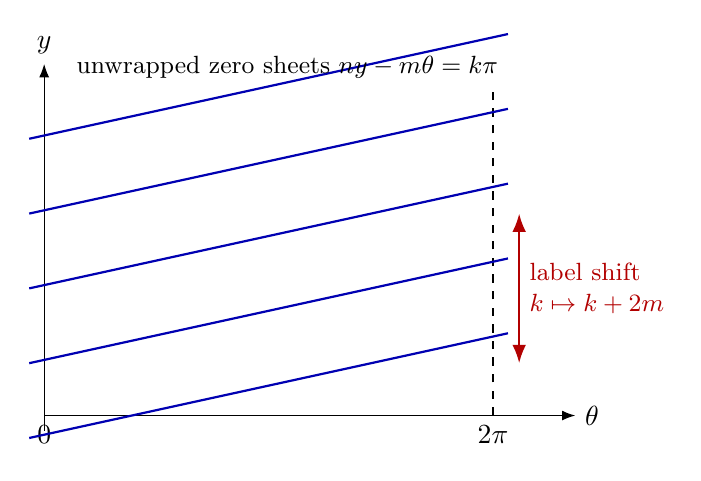
\begin{tikzpicture}[x=0.95cm,y=0.95cm,>=Latex]
  \draw[->] (0,0)--(7.1,0) node[right] {$\theta$};
  \draw[->] (0,-0.2)--(0,4.7) node[above] {$y$};
  \draw[dashed] (6,0)--(6,4.4);
  \node[below] at (0,0) {$0$};
  \node[below] at (6,0) {$2\pi$};
  \foreach \j in {-1,0,1,2,3} {
    \draw[blue!70!black,thick] (-0.2,{0.7+1.0*\j}) -- (6.2,{2.1+1.0*\j});
  }
  \draw[<->,red!70!black,thick] (6.35,0.7)--(6.35,2.7)
    node[midway,right,align=left,font=\small]{label shift\\$k\mapsto k+2m$};
  \node[align=center,font=\small] at (3.25,4.65)
    {unwrapped zero sheets $ny-m\theta=k\pi$};
\end{tikzpicture}
\caption{The helical tube on the unwrapped $(\theta,y)$-plane.  Vertical boundary
identification at $\theta=0,2\pi$ produces the permutation
\eqref{eq:helical-permutation}; the drawing is schematic, while the slope is fixed
exactly by $\dd y/\dd\theta=m/n$.}
\label{fig:helical-unwrapped}
\end{figure}

\subsection{Boundary traces and logarithmic sheets}

At either boundary component $x=\pm L$, the trace lies in the parameter-position
torus $S^1_\theta\times S^1_y$ and satisfies
\[
 ny-m\theta\in\pi\Z.
\]
It has $2d$ connected components.  Each is a primitive curve with homology class
\begin{equation}
 \frac nd[S^1_\theta]+\frac md[S^1_y].
 \label{eq:helical-boundary-class}
\end{equation}
If $T(p,q)$ denotes the torus link whose total homology data in these ordered
coordinates are $(p,q)$, the full trace is $T(2n,2m)$, up to simultaneous
orientation reversal.  This statement depends on the declared torus coordinates;
it is not an intrinsic knot type before an embedding of that torus in a
three-manifold is fixed.

Unwrap the $y$-circle to $y\in\R$.  Formula~\eqref{eq:helical-zero-fiber} now has
labels $k\in\Z$.  The parameter loop sends $k\mapsto k+2m$, while the deck
transformation $y\mapsto y+2\pi$ sends $k\mapsto k+2n$.  The finite downstairs
system is exactly the quotient of this countable label set by the deck action.
This simultaneously realizes a proper tube and a nontrivial logarithmic shift.

\begin{corollary}[Finite quotient of the helical lift]
\label{cor:helical-finite-quotient}
For the helical family, the countable lifted sheets contain no additional
component permutation beyond the affine action generated by the two translations
$2m$ and $2n$ on $\Z$.  Downstairs component monodromy is their reduction modulo
$2n$.
\end{corollary}

\subsection{Embedded monodromy versus braid monodromy}

The permutation \eqref{eq:helical-permutation} is honest monodromy, but it is not
an element of $B_{2n}$.  Its fiber consists of intervals in a surface, not points in
a disc.  Intersecting the zero tube with $x=c$ produces a one-dimensional trace in
$S^1_y\times S^1_\theta$, but the choice of $c$ is additional probe data.  Section
\ref{sec:threading} formalizes this distinction.

Even for compact circle fibers in Theorem~\ref{thm:proper-real-zero-tube}, the
abstract monodromy of the one-manifold fiber records only a permutation and
orientation-preserving return maps of circles.  The embedding in the ambient
surface can carry a richer mapping class, but that is a mapping-class problem for
curves, not the ordinary braid group of moving points.


\section{Singular fibers and branched fillings}
\label{sec:singular-fibers}
\subsection{Real Morse events in the singular category}

Let $\tau\in\R$ and consider the two functions
\begin{equation}
 a^+_\tau(x,y)=x^2+y^2-\tau,
 \qquad
 a^-_\tau(x,y)=x^2-y^2-\tau.
 \label{eq:morse-assignments}
\end{equation}
Their common critical set in each slice is the origin.  On
$\R^2\setminus\{0\}$ define
\begin{equation}
 g^\pm_\tau=
 \frac{4(x^2+y^2)}
 {\mu^2+\lambda^2(a^\pm_\tau)^2}
 (\dd x^2+\dd y^2).
 \label{eq:morse-aeg-metric}
\end{equation}

\begin{proposition}[AEG Morse bifurcations]
\label{prop:aeg-morse-bifurcations}
For every $\tau$, the tuple
\[
 (\R^2,\{0\},g^\pm_\tau,a^\pm_\tau;\mu,\lambda)
\]
is a singular AES.  Its total zero incidence in $\R^2\times\R_\tau$ is smooth,
but projection to $\tau$ has a critical point at $(0,0,0)$.

For $a^+_\tau$, the zero changes from empty to a singular point and then to a
circle as $\tau$ crosses zero.  For $a^-_\tau$, the two hyperbolic branches
reconnect through the four regular rays meeting at the singular origin when
$\tau=0$.
\end{proposition}

\begin{proof}
The Euclidean norm squared of $\dd a^\pm_\tau$ is $4(x^2+y^2)$, so
Corollary~\ref{cor:singular-realization} gives the AEG equation and local
essentiality.  Define
$A^\pm(x,y,\tau)=a^\pm_\tau(x,y)$.  Since
$\partial_\tau A^\pm=-1$, zero is a regular value of the total function; hence
$(A^\pm)^{-1}(0)$ is smooth.  The parameter projection restricted to it is
critical precisely when the spatial derivative vanishes, which happens at the
origin.  The stated zero sets follow directly from
$x^2+y^2=\tau$ and $x^2-y^2=\tau$.
\end{proof}

\begin{figure}[ht]
\centering
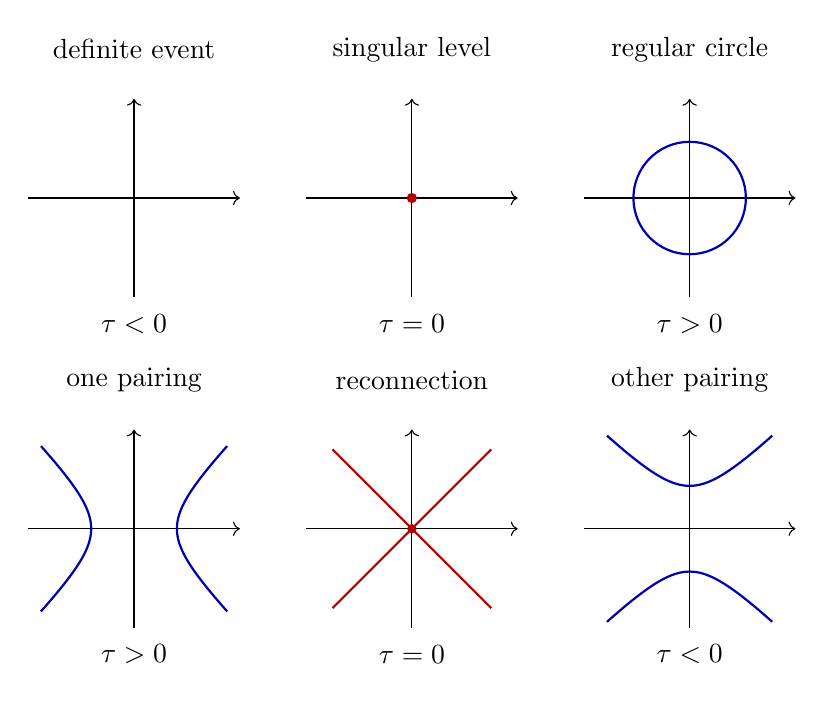
\begin{tikzpicture}[scale=0.84]
  \begin{scope}[xshift=0cm]
    \node at (0,2.25) {definite event};
    \draw[->] (-1.6,0)--(1.6,0);
    \draw[->] (0,-1.5)--(0,1.5);
    \node at (0,-1.9) {$\tau<0$};
  \end{scope}
  \begin{scope}[xshift=4.2cm]
    \node at (0,2.25) {singular level};
    \draw[->] (-1.6,0)--(1.6,0);
    \draw[->] (0,-1.5)--(0,1.5);
    \fill[red!70!black] (0,0) circle (2.2pt);
    \node at (0,-1.9) {$\tau=0$};
  \end{scope}
  \begin{scope}[xshift=8.4cm]
    \node at (0,2.25) {regular circle};
    \draw[->] (-1.6,0)--(1.6,0);
    \draw[->] (0,-1.5)--(0,1.5);
    \draw[blue!70!black,thick] (0,0) circle (0.85);
    \node at (0,-1.9) {$\tau>0$};
  \end{scope}
  \begin{scope}[yshift=-5.0cm]
    \node at (0,2.25) {one pairing};
    \draw[->] (-1.6,0)--(1.6,0);
    \draw[->] (0,-1.5)--(0,1.5);
    \draw[blue!70!black,thick,domain=-1.25:1.25,samples=80]
      plot ({sqrt(0.42+\x*\x)},\x);
    \draw[blue!70!black,thick,domain=-1.25:1.25,samples=80]
      plot ({-sqrt(0.42+\x*\x)},\x);
    \node at (0,-1.9) {$\tau>0$};
  \end{scope}
  \begin{scope}[xshift=4.2cm,yshift=-5.0cm]
    \node at (0,2.25) {reconnection};
    \draw[->] (-1.6,0)--(1.6,0);
    \draw[->] (0,-1.5)--(0,1.5);
    \draw[red!70!black,thick] (-1.2,-1.2)--(1.2,1.2);
    \draw[red!70!black,thick] (-1.2,1.2)--(1.2,-1.2);
    \fill[red!70!black] (0,0) circle (2pt);
    \node at (0,-1.9) {$\tau=0$};
  \end{scope}
  \begin{scope}[xshift=8.4cm,yshift=-5.0cm]
    \node at (0,2.25) {other pairing};
    \draw[->] (-1.6,0)--(1.6,0);
    \draw[->] (0,-1.5)--(0,1.5);
    \draw[blue!70!black,thick,domain=-1.25:1.25,samples=80]
      plot (\x,{sqrt(0.42+\x*\x)});
    \draw[blue!70!black,thick,domain=-1.25:1.25,samples=80]
      plot (\x,{-sqrt(0.42+\x*\x)});
    \node at (0,-1.9) {$\tau<0$};
  \end{scope}
\end{tikzpicture}
\caption{Real AEG-compatible Morse examples.  The red point is a declared
essential singularity.  The pictures record zero topology only; they are not a
classification of metric germs.}
\label{fig:real-morse-events}
\end{figure}

The proposition exhibits the key phenomenon
\[
 \text{smooth total zero incidence}
 \not\!\Longrightarrow
 \text{zero tube}.
\]
At the event, it is the projection that fails to be a submersion.

\subsection{A regular-to-singular fold wall}

A related family makes all noncritical slices regular rather than retaining a
singular point away from the zero.  Put
\[
 A(x,y,\tau)=e^x(y^2-\tau).
\]
For $\tau\ne0$, the spatial derivative never vanishes; for $\tau=0$, it vanishes
along the entire line $y=0$.  On the regular locus use
\begin{equation}
 g_\tau=
 \frac{e^{2x}\bigl((y^2-\tau)^2+4y^2\bigr)}
 {\mu^2+\lambda^2e^{2x}(y^2-\tau)^2}
 (\dd x^2+\dd y^2).
 \label{eq:fold-wall-metric}
\end{equation}
For $\tau<0$ the zero fiber is empty, for $\tau>0$ it consists of two parallel
lines, and for $\tau=0$ it is the singular line $y=0$.  The metric degenerates
there and the line is locally essential.  This is a verified wall-crossing family,
but it is nonproper and its singular stratum is one-dimensional.

\subsection{The complex branch model}

Real scalar zeros and complex roots have different local models.  Let
$(w,\tau)\in\C^2$ and consider
\begin{equation}
 F(w,\tau)=w^2-\tau.
 \label{eq:complex-branch-model}
\end{equation}
The incidence $F^{-1}(0)$ is a smooth complex curve parameterized by
$w\mapsto(w,w^2)$.  Its projection to the $\tau$-plane is a two-sheeted branched
cover with a single simple branch point at the origin.

On the boundary circle $\tau=\varepsilon e^{i\theta}$, the two roots are
\begin{equation}
 w_\pm(\theta)=\pm\sqrt\varepsilon\,e^{i\theta/2}.
 \label{eq:half-twist-roots}
\end{equation}
They remain distinct for every boundary parameter and exchange after one circuit.
The boundary therefore carries the standard half-twist in $B_2$; the collision is
at the center of the filling, not on the boundary braid.

\begin{proposition}[Simple polynomial discriminant normal form]
\label{prop:simple-discriminant-normal-form}
Let a holomorphic family of monic polynomials, parameterized by a complex
$d$-manifold, meet the polynomial discriminant transversely at a parameter where
exactly one root has multiplicity two and all other roots are simple.  After
holomorphic changes of root and parameter coordinates
$\tau=(\tau_1,\ldots,\tau_d)$, its local root incidence is the disjoint union of
simple graphs and one copy of
\[
 w^2=\tau_1,
\]
with $\tau_2,\ldots,\tau_d$ as spectator coordinates.
\end{proposition}

\begin{proof}
Separate the simple roots by the holomorphic implicit-function theorem.  The
remaining quadratic factor has the form $w^2+b(\tau)w+c(\tau)$.  Translating
$w$ removes the linear term.  Its discriminant is a holomorphic function of the
parameter; transversality makes that function the first member $\tau_1$ of a
local coordinate system.  Rescaling $\tau_1$ gives
\eqref{eq:complex-branch-model}, while the remaining parameter coordinates pass
through unchanged.
\end{proof}

Restricting $\tau$ to the real axis gives two real roots for $\tau>0$ and two
imaginary roots for $\tau<0$.  Their four half-arcs meet at the branch point.  This
four-valent picture is a real slice of a complex branched cover, not a regular
four-valent zero of a real assignment.

\subsection{Smooth and holomorphic fillings}

Section~\ref{sec:braids} realizes every braid by a family that is smooth in the
loop parameter and holomorphic in the spatial coordinate $w$.  Extending such a
family over a parameter disc while remaining holomorphic in both variables is a
stronger demand.  Algebraic-function boundaries are constrained by
quasipositivity \cite{Rudolph1983AlgebraicFunctions}.  Thus the statements
\begin{align*}
 &\text{every braid has an arithmetic-holomorphic spatial realization},\\
 &\text{every braid bounds a holomorphic AEG root filling}
\end{align*}
are not equivalent; the first is proved below, while the second is false without
restrictions.

\begin{problem}[AEG-natural singular fillings]
\label{prob:natural-fillings}
Determine which branch signs and global braided surfaces arise when the parameter
dependence is constrained by expression history or by a natural connection, rather
than chosen as an arbitrary smooth or holomorphic polynomial family.
\end{problem}


\section{Complex roots, monodromy, and braids}
\label{sec:braids}
\subsection{Square-free polynomials as a finite-root interface}

Let $\mathcal P_n\cong\C^n$ be the space of monic degree-$n$ complex
polynomials and let $\Delta_n\subset\mathcal P_n$ be its algebraic discriminant.
The square-free locus is
\[
 \sfP_n=\mathcal P_n\setminus\Delta_n.
\]
Vieta's map identifies it with the unordered configuration space
\begin{equation}
 \sfP_n\cong\UConf_n(\C)
 =\Conf_n(\C)/S_n.
 \label{eq:vieta-configuration}
\end{equation}
Its fundamental group is the Artin braid group $B_n$
\cite{Artin1925TheorieDerZoepfe,FadellNeuwirth1962ConfigurationSpaces,Birman1974Braids}.

\begin{theorem}[Finite-root incidence and braid monodromy]
\label{thm:finite-root-braid}
Let $B$ be a connected smooth manifold and let
\begin{equation}
 F_b(w)=w^n+c_1(b)w^{n-1}+\cdots+c_n(b)
 \label{eq:polynomial-family}
\end{equation}
be a smooth family of monic polynomials with nonvanishing discriminant.  Then
\begin{equation}
 \calR_F=\{(w,b)\in\C\times B:F_b(w)=0\}
 \label{eq:root-incidence}
\end{equation}
is a smooth real codimension-two submanifold whose
projection to $B$ is a proper $n$-sheeted covering.  The coefficient map
$c:B\to\sfP_n$ induces
$c_*:\pi_1(B,b_0)\to\pi_1(\sfP_n,c(b_0))$.  After choosing the usual path to a
standard base configuration and the resulting identification of the target with
$B_n$, this is braid monodromy
\begin{equation}
 c_*:\pi_1(B,b_0)\longrightarrow B_n.
 \label{eq:braid-monodromy-map}
\end{equation}
Changing that identification conjugates the representation.
Its composition with $B_n\to S_n$ is the ordinary permutation monodromy of the
covering $\calR_F\to B$.
\end{theorem}

\begin{proof}
At a root of a square-free polynomial,
$\partial F_b/\partial w\ne0$.  The implicit-function theorem therefore writes the
root incidence locally as $n$ disjoint graphs over $B$, so it is an $n$-sheeted
covering.  A finite covering of locally compact Hausdorff spaces is proper.  The
map to unordered root configurations is exactly the coefficient map under
\eqref{eq:vieta-configuration}; functoriality of the fundamental group gives
\eqref{eq:braid-monodromy-map}.  Forgetting paths and retaining only their endpoint
labels is the standard quotient $B_n\to S_n$.
\end{proof}

For $B=S^1$, the incidence is a closed geometric braid in
$\C\times S^1$.  A basepoint and an ordering above it give an element of $B_n$;
changing the basepoint or ordering conjugates that element.  This is strictly more
information than the endpoint permutation.

\begin{warning}[Rank-one assignments do not yield $B_n$]
\label{warn:rank-one-not-braid}
The field $F$ in Theorem~\ref{thm:finite-root-braid} is complex-valued and has real
rank two.  The theorem does not turn a real AEG assignment into a polynomial, nor
does it promote a moving family of zero curves to a finite-root braid.  The two
constructions share the parameterized zero-section theorem but have different
codimensions.
\end{warning}

\subsection{Arithmetic-holomorphic braid realization}

On the complete basic hyperbolic AES with $\mu,\lambda>0$, Paper II constructs a global coordinate
$w=X+iy\in\HH$ in which arithmetic holomorphicity is ordinary holomorphicity.
This supplies a precise AEG background for Theorem~\ref{thm:finite-root-braid}.

\begin{theorem}[AEG realization of every braid]
\label{thm:aeg-braid-realization}
For every $\beta\in B_n$ and every complete basic hyperbolic AES with
$\mu,\lambda>0$, there is a smooth loop of arithmetic-holomorphic fields
$F_\theta$ such that:
\begin{enumerate}
\item every $F_\theta$ is a monic degree-$n$ polynomial in the arithmetic
holomorphic coordinate $w$;
\item all roots lie in a fixed disc $D\Subset\HH$ and remain simple;
\item the root incidence realizes the geometric braid $\beta$.
\end{enumerate}
Consequently, every oriented link is the closure of the root incidence of such an
arithmetic-holomorphic family.
\end{theorem}

\begin{proof}
Represent $\beta$ by a smooth loop
$\{z_1(\theta),\ldots,z_n(\theta)\}$ in
$\UConf_n(\C)$.  On the parameter interval $[0,2\pi]$, choose a smooth ordered
lift $(z_1(\theta),\ldots,z_n(\theta))$; its two endpoints may differ by the
permutation underlying $\beta$.  An affine translation and positive rescaling
place the compact unordered image in a disc $D\Subset\HH$ without changing its
braid class.  Set
\begin{equation}
 F_\theta(w)=\prod_{j=1}^n\bigl(w-z_j(\theta)\bigr).
 \label{eq:aeg-braid-polynomial}
\end{equation}
Because the endpoint lists differ only by a permutation, the coefficients are
smooth and periodic in $\theta$.  The roots are simple, and
each slice is holomorphic in $w$.  Paper II identifies it as an
arithmetic-holomorphic field.  Its root incidence is the chosen loop of
configurations.  The last statement follows from Alexander's closed-braid theorem
\cite{Alexander1923KnottedCurves}.
\end{proof}

The theorem is a universality result, not an invariant.  Because every braid can
be realized, the predicate ``admits an AEG root-tube realization'' cannot
distinguish links.  New information would have to be supplied by a natural
history-derived decoration or by a restricted class of allowed families.

\subsection{Logarithmic lifting of root tubes}

Suppose all roots avoid the origin.  Pull the root incidence back along
$\exp:\C\to\C^\times$:
\begin{equation}
 \widetilde{\calR}_F
 =\{(b,\omega):F_b(e^\omega)=0\}.
 \label{eq:log-root-incidence}
\end{equation}

\begin{theorem}[Logarithmic root transport and gauge]
\label{thm:log-root-transport}
The map $\widetilde{\calR}_F\to\calR_F$ is the canonical principal
$2\pi i\Z$-cover obtained by pullback of the exponential cover.  Its specified
deck-translation action is $\omega\mapsto\omega+2\pi i k$.  Along a parameter
loop, choose a labeling of the initial roots and
logarithmic lifts.  If root continuation has permutation $\sigma$, then there are
integers $k_i$ such that
\begin{equation}
 \omega_i(1)=\omega_{\sigma(i)}(0)+2\pi i k_i.
 \label{eq:log-endpoint-shift}
\end{equation}
Changing the initial lifts by
$\omega_i(0)\mapsto\omega_i(0)+2\pi i m_i$ changes the integers by
\begin{equation}
 k_i\longmapsto k_i+m_i-m_{\sigma(i)}.
 \label{eq:log-gauge-law}
\end{equation}
For every cycle of $\sigma$, the sum of the $k_i$ on that cycle is gauge invariant.
Relabeling the roots permutes these cycle sums, so their multiset, rather than an
ordered list, is label-independent.  The total sum $\sum_i k_i$ is gauge and label
invariant and equals the winding of the product of the roots around zero.
\end{theorem}

\begin{proof}
Equation~\eqref{eq:log-root-incidence} is the pullback of the exponential cover,
so the first claim is immediate.  Unique path lifting gives
\eqref{eq:log-endpoint-shift}.  If the initial lift of the $i$th path is shifted by
$2\pi im_i$, its entire lift is shifted by that amount.  Comparing the new endpoint
with the new lift assigned to the root $\sigma(i)$ gives
\eqref{eq:log-gauge-law}.  The $m_i$ terms telescope around each permutation cycle.
Finally, the product of all roots is, up to sign, the constant coefficient of
$F_b$; summing logarithmic increments computes its winding.
\end{proof}

Thus a vector $(k_i)$ is not an invariant before a lift gauge is fixed.  Cycle sums
are invariant but abelian.  The full noncommutative information remains in the
configuration path, more precisely in the annular braid group when roots are
constrained to $\C^\times$.

\subsection{Boundary braid and discriminant filling}

Theorem~\ref{thm:finite-root-braid} applies only in the complement of
$\Delta_n$.  A filling disc may meet the discriminant.  At a transverse simple
intersection, Proposition~\ref{prop:simple-discriminant-normal-form} gives
$w^2=\tau$, and its boundary loop contributes a conjugate of a standard positive
or negative half-twist according to orientation.  The collision is therefore a
two-cell event in the filling, while the boundary braid stays collision-free.

This separation resolves an otherwise persistent ambiguity:
\begin{center}
\small
\begin{tabular}{lll}
\toprule
Object & Allowed local event & Output \\
\midrule
regular real assignment family & no critical zero & curve tube \\
singular real family & Morse critical zero & birth or reconnection \\
square-free boundary root family & no repeated root & braid monodromy \\
root filling through $\Delta_n$ & simple double root & branch half-twist \\
\bottomrule
\end{tabular}
\end{center}

\begin{problem}[Natural braid monodromy]
\label{prob:natural-braid-monodromy}
Find a functorial procedure that assigns a finite complex-root field to an
expression history or to a real zero tube, and prove that the resulting braid is
independent of auxiliary coordinates and probes.  The arbitrary polynomial
realization of Theorem~\ref{thm:aeg-braid-realization} does not solve this problem.
\end{problem}


\section{Threading, affine torsion, and the knot frontier}
\label{sec:threading}
\subsection{Threads are additional data}

The real zero tube has curve fibers.  To obtain moving points one must select them.

\begin{definition}[Finite zero thread]
\label{def:finite-zero-thread}
Let $\pi:\calZ\to B$ be an embedded real zero tube over a connected
one-manifold.  A \emph{finite zero thread} is a properly embedded
one-dimensional submanifold $K\subset\calZ$, with
$\partial K=K\cap\pi^{-1}(\partial B)$ when the base has boundary, such that
$\pi|_K:K\to B$ is a finite-sheeted covering.  For $B=S^1$, this forces $K$ to be
a compact one-manifold without boundary.  The pair $(\calZ,K)$ is a
\emph{threaded zero tube}.  A thread is \emph{intrinsic} only if its construction
from the stated AEG data is functorial under the declared notion of AEG
isomorphism.
\end{definition}

In the helical family, every slice $x=c$ gives
\[
 K_c=\calZ(A_{m,n})\cap\{x=c\},
\]
a degree-$2n$ finite thread.  Its homology and component structure are computed in
\eqref{eq:helical-boundary-class}.  The choice of $c$ is a probe choice; if one uses
$c=\pm L$, the boundary is part of the domain data but the choice of boundary
component remains.  Selecting only one of the $2d$ components is another choice.

A rank-two root incidence such as $\calR_F$ is already one-dimensional, so it plays
the role of its own finite thread.  If its moving points lie in a disc, it is an
ordinary geometric braid.  If they lie in an annulus or general surface, the
relevant surface braid group and equivalence relation must be named.

\subsection{A scalar Markov obstruction}

The first novelty filter is independent of AEG.

\begin{proposition}[Stateless additive collapse]
\label{prop:stateless-additive-collapse}
Let $A$ be an abelian group and $n\ge2$.  Every homomorphism
$\Theta_n:B_n\to A$ factors through the exponent sum (writhe)
$w:B_n\to\Z$:
\[
 \Theta_n(\beta)=w(\beta)c_n
\]
for a fixed $c_n\in A$.  If the family $\Theta_n$ is compatible with the standard
inclusions $B_n\hookrightarrow B_{n+1}$ and is unchanged under both Markov
stabilizations $\beta\mapsto\beta\sigma_n^{\pm1}$, then every $\Theta_n$ is zero.
\end{proposition}

\begin{proof}
In an abelian target, the braid relation
$\sigma_i\sigma_{i+1}\sigma_i=\sigma_{i+1}\sigma_i\sigma_{i+1}$ implies
$\Theta_n(\sigma_i)=\Theta_n(\sigma_{i+1})$.  All standard generators therefore
have the same image $c_n$, and the homomorphism is exponent sum times $c_n$.
Inclusion compatibility identifies $c_n$ with $c_{n+1}$.  Positive stabilization
then gives $c_{n+1}=0$; negative stabilization gives the same conclusion.  Hence
the family vanishes.
\end{proof}

Allowing a normalization depending on strand number does not evade both signs.  If
$I_n(\beta)=c\,w(\beta)+d n$ in an additive coefficient group, positive and
negative stabilization require $c+d=0$ and $-c+d=0$.  Away from two-torsion this
forces $c=d=0$, and in all cases it leaves no noncommutative information.  A useful
AEG invariant must retain state, use a trace-like normalization, or belong to a
more structured category.

\subsection{Affine conjugation and the Alexander layer}

Let $R$ be a commutative ring.  Write an affine transformation as $(p,u)$, with
$p\in R^\times$ and $u\in R$, acting by $x\mapsto px+u$.  Thus all multipliers
$p,q,r$ below are units and all translation coordinates $u,v,w$ lie in $R$.  We use
\begin{equation}
 (p,u)(q,v)=(pq,u+pv),
 \qquad
 (p,u)^{-1}=(p^{-1},-p^{-1}u).
 \label{eq:affine-group-law}
\end{equation}
Right conjugation $x\triangleright y=y^{-1}xy$ is
\begin{equation}
 (p,u)\triangleright(q,v)
 =\left(p,q^{-1}\bigl(u+(p-1)v\bigr)\right).
 \label{eq:affine-conjugation}
\end{equation}
On the fixed-multiplier branch
$X_t=\{(t,u):u\in R\}$ over a commutative ring in which $t$ is a unit, this becomes
\begin{equation}
 u\triangleright v=t^{-1}u+(1-t^{-1})v.
 \label{eq:alexander-quandle-operation}
\end{equation}
It is exactly an Alexander quandle, not a structure beyond the Alexander layer.

The affine torsion expression
\begin{equation}
 \kappa\bigl((p,u),(q,v)\bigr)=(1-q)u+(p-1)v
 \label{eq:affine-torsion}
\end{equation}
restricts to
\begin{equation}
 \kappa_t(u,v)=(t-1)(v-u).
 \label{eq:fixed-torsion}
\end{equation}

\begin{proposition}[Ordinary exactness]
\label{prop:ordinary-affine-exactness}
With the ordinary quandle coboundary convention
$df(x,y)=f(x\triangleright y)-f(x)$, one has
\[
 \kappa_t=d(tf)
 \qquad\text{for }f(u)=u.
\]
Thus the fixed-multiplier affine torsion represents the zero ordinary quandle
cohomology class.
\end{proposition}

\begin{proof}
Equation~\eqref{eq:alexander-quandle-operation} gives
\[
 df(u,v)=(t^{-1}-1)u+(1-t^{-1})v
 =\frac{t-1}{t}(v-u).
\]
Multiplication by $t$ gives \eqref{eq:fixed-torsion}.
\end{proof}

\subsection{Twisting, resonance, and a nonzero class}

We now use the twisted convention of Carter--Elhamdadi--Saito
\cite{CarterElhamdadiSaito2002TwistedQuandle}.  Let the coefficient action be a
scalar $T_{\mathrm{coef}}$.  A normalized twisted $2$-cocycle $\phi$ satisfies
\begin{align}
 T_{\mathrm{coef}}\phi(x,y)+\phi(x\triangleright y,z)
 ={}&T_{\mathrm{coef}}\phi(x,z)
 +(1-T_{\mathrm{coef}})\phi(y,z)\notag\\
 &+\phi(x\triangleright z,y\triangleright z),
 \label{eq:twisted-cocycle-equation}
\end{align}
and $\phi(x,x)=0$.  For coboundaries we choose the sign
\begin{equation}
 \delta_T^+f(x,y)=T_{\mathrm{coef}}f(x)
 +(1-T_{\mathrm{coef}})f(y)-f(x\triangleright y).
 \label{eq:twisted-coboundary-convention}
\end{equation}
The chain-level convention in the cited paper differs from
\eqref{eq:twisted-coboundary-convention} by a global minus sign in one displayed
definition, while its extension and state-sum calculations use the sign above.
The coboundary subgroup is the same under either choice.

Put $\alpha=t^{-1}$.  Direct substitution in
\eqref{eq:twisted-cocycle-equation} shows that $\kappa_t$ is a twisted cocycle for
every coefficient action.  If $\alpha-T_{\mathrm{coef}}$ is a unit in the
coefficient ring, it is exact: for
\[
 f(u)=\frac{t-1}{\alpha-T_{\mathrm{coef}}}u
\]
one has $\delta_T^+f=\kappa_t$.  Over a field, only the resonance
$T_{\mathrm{coef}}=\alpha$ survives this linear exactness test; over a general ring,
a nonzero nonunit difference may also obstruct this particular linear primitive.

\begin{theorem}[Finite-field resonant affine class]
\label{thm:resonant-affine-class}
Let $q$ be a prime power, let
$t\in\F_q^\times\setminus\{1\}$, and put $\alpha=t^{-1}$.  Give
$X_t=\F_q$ the Alexander operation
$x\triangleright y=\alpha x+(1-\alpha)y$ and give the coefficient module
$N=\F_q$ the resonant action $T_{\mathrm{coef}}=\alpha$.  Then
\begin{equation}
 \kappa_t(x,y)=(t-1)(y-x)
 \label{eq:finite-field-kappa}
\end{equation}
is a normalized twisted $2$-cocycle representing a nonzero class in
$H^2_{TQ}(X_t;N)$.
\end{theorem}

\begin{proof}
Normalization is immediate, and substituting the Alexander operation into
\eqref{eq:twisted-cocycle-equation} makes both sides equal
\[
 (t-1)\bigl[z-(\alpha+T_{\mathrm{coef}})x
 +(\alpha+T_{\mathrm{coef}}-1)y\bigr].
\]
Suppose $\kappa_t=\delta_T^+f$.  Subtracting the constant $f(0)$ does not change
the coboundary, so take $g(0)=0$.  Setting $y=0$ gives
\begin{equation}
 g(\alpha x)-\alpha g(x)=(t-1)x.
 \label{eq:resonant-recurrence}
\end{equation}
Let $r=\ord(\alpha)$.  Iterating \eqref{eq:resonant-recurrence} yields
\[
 g(\alpha^r x)=\alpha^r g(x)+r(t-1)\alpha^{r-1}x.
\]
But $\alpha^r=1$ and $r$ divides $q-1$, so the characteristic of $\F_q$ does not
divide $r$.  Taking $x\ne0$ contradicts $t\ne1$.  Hence no one-cochain has
coboundary $\kappa_t$.
\end{proof}

This closes the algebraic resonance question, but it does not yet produce a
stronger classical knot invariant.  In fact, a second calculation gives a sharp
collapse theorem.

We now fix the precise planar state-sum convention.  Give each oriented arc the
normal for which the ordered pair (tangent, normal) agrees with the plane
orientation, and give the unbounded region Alexander number zero.  At a crossing
$\tau$, let $L(\tau)$ be the Alexander number of the source region from which both
arc normals point.  Let $y_\tau$ be the over-arc color, and let its normal point
from an under-arc colored $x_\tau$ to one colored
$x_\tau\triangleright y_\tau$.  Define $\epsilon(\tau)=1$ when the ordered pair
(over-arc normal, under-arc normal) agrees with the plane orientation and
$\epsilon(\tau)=-1$ otherwise.  In additive coefficient notation the twisted
Boltzmann weight is
\begin{equation}
 B_T(\tau,C)=
 T_{\mathrm{coef}}^{-L(\tau)}
 \bigl(\epsilon(\tau)\kappa_t(x_\tau,y_\tau)\bigr)\in N,
 \label{eq:twisted-boltzmann-weight}
\end{equation}
and the state sum is
\begin{equation}
 \Phi_{\kappa_t}(D)
 =\sum_{C\in\operatorname{Col}_{X_t}(D)}
  \left[\sum_{\tau}B_T(\tau,C)\right]\in\Z[N].
 \label{eq:twisted-state-sum}
\end{equation}
Here $[a]$ denotes the basis element of the integral group ring indexed by
$a\in N$.  This is the additive form of the standard twisted convention.

\begin{theorem}[Planar state-sum collapse]
\label{thm:resonant-state-sum-collapse}
Under the hypotheses of Theorem~\ref{thm:resonant-affine-class}, the standard
twisted quandle cocycle state sum \eqref{eq:twisted-state-sum} is a Reidemeister
invariant of oriented classical links, but for every planar link diagram $D$ it is
\begin{equation}
 \Phi_{\kappa_t}(D)=
 \bigl|\operatorname{Col}_{X_t}(D)\bigr|[0].
 \label{eq:planar-state-sum-collapse}
\end{equation}
Thus it provides no enhancement of the Alexander quandle coloring count.
\end{theorem}

\begin{proof}
The Reidemeister invariance follows from the standard twisted-cocycle theorem
\cite{CarterElhamdadiSaito2002TwistedQuandle}.  To identify the value, define the
two-dimensional $\F_q$-vector space $E=N\oplus X_t$ with Laurent action
\begin{equation}
 T_E(a,x)=\bigl(\alpha a-(t-1)x,\alpha x\bigr).
 \label{eq:extension-action}
\end{equation}
This is invertible and makes
$0\to N\to E\to X_t\to0$ a short exact sequence of Alexander modules.  For the
section $s(x)=(0,x)$,
\begin{equation}
 T_Es(x)+(1-T_E)s(y)-s(x\triangleright y)
 =\bigl(\kappa_t(x,y),0\bigr).
 \label{eq:kappa-obstruction}
\end{equation}
Hence $\kappa_t$ is the obstruction cocycle of an Alexander-module extension.
The planar obstruction-cocycle cancellation theorem of
Carter--Elhamdadi--Saito then makes every coloring contribute the identity weight.
With convention \eqref{eq:twisted-state-sum}, the state sum is therefore exactly
$|\operatorname{Col}_{X_t}(D)|[0]$.
\end{proof}

Theorems~\ref{thm:resonant-affine-class} and
\ref{thm:resonant-state-sum-collapse} illustrate why cohomological nontriviality
and knot-theoretic detection must be tested separately.  A nonzero class can have a
trivial planar enhancement because its weights cancel through an extension.
On diagrams in nonplanar surfaces, the same extension argument need not cancel;
that is a different, surface-link question and is not promoted here to an ordinary
$S^3$ invariant.

\subsection{Variable multipliers and the Reidemeister-III anomaly}

For the full affine quandle, the torsion
\eqref{eq:affine-torsion} is generally not an ordinary $2$-cocycle.  With
$x=(p,u)$, $y=(q,v)$, and $z=(r,w)$, define its type-III defect by
\begin{align*}
 \mathfrak A_\kappa(x,y,z)
 ={}&\kappa(x,y)+\kappa(x\triangleright y,z)
 -\kappa(x,z)-\kappa(x\triangleright z,y\triangleright z).
\end{align*}
A direct calculation gives
\begin{equation}
 \mathfrak A_\kappa(x,y,z)
 =\frac{(q-r)(r-1)}{qr}\,\kappa(x,y).
 \label{eq:variable-multiplier-anomaly}
\end{equation}
It vanishes on a fixed-multiplier branch, as it must.  On a one-component knot,
conjugate meridians also have equal multipliers, so arbitrary multiplier variation
along arcs is not legitimate coloring data.  Nonzero use of
\eqref{eq:variable-multiplier-anomaly} would require additional region state, a
multi-component setting, a dynamical quandle, or another declared structure.

\begin{warning}[Anomaly is not associator]
A failure of the ordinary type-III cocycle equation is not automatically a higher
associator or a surface-holonomy invariant.  Such an interpretation requires
separate pentagon/hexagon or equivalent coherence and filling-independence proofs.
\end{warning}

\subsection{A historical free-word calculation}

One useful repository computation can be stated without overclaiming it.  Use the
historical figure-eight knot-group presentation
\[
 G_{4_1}=\langle a,b\mid abbbaBAAB=1\rangle,
 \qquad A=a^{-1},\quad B=b^{-1}.
\]
Under
the convention that $a:x\mapsto tx$, $b:x\mapsto x+1$, uppercase letters denote
inverses, and the displayed transformations compose in the fixed word order, the
free-group word
\[
 abbbaBAAB
\]
has unit multiplier and translation coordinate
\begin{equation}
 -\Delta_{4_1}(t)=-(t^2-3t+1).
 \label{eq:figure-eight-free-word}
\end{equation}
This is a verified affine word calculation.  The displayed generator assignment
descends from the free group to $G_{4_1}$ only on the parameter locus
$\Delta_{4_1}(t)=0$.  At generic $t$ it is not a knot invariant; it is the failure
of the chosen generator assignment to satisfy the relator.

\subsection{The remaining invariant gate}

Theorem~\ref{thm:aeg-braid-realization} supplies every braid, and
Definition~\ref{def:finite-zero-thread} supplies explicit threads in selected real
tubes.  Neither result selects a choice-free numerical or algebraic decoration.
For a family $I_n:B_n\to\mathcal A$ to descend to oriented links via Markov's
theorem, it must at minimum satisfy
\begin{equation}
\begin{aligned}
 I_n(\gamma\beta\gamma^{-1})&=I_n(\beta),\\
 I_{n+1}(\iota_n\beta\,\sigma_n)&=I_n(\beta),\\
 I_{n+1}(\iota_n\beta\,\sigma_n^{-1})&=I_n(\beta).
\end{aligned}
\label{eq:markov-gate}
\end{equation}
after any declared normalization \cite{Birman1974Braids}.  An AEG construction
must additionally prove independence of logarithmic lift, probe, thread, spine,
axis, basepoint, and expression presentation whenever those are auxiliary choices.

\begin{problem}[AEG Markov descent]
\label{prob:aeg-markov-descent}
Construct a nonabelian or stateful decoration natural under AEG isomorphisms, prove
the braid relations and all choice-independence statements, and find a Markov
normalization satisfying \eqref{eq:markov-gate}.
\end{problem}

\begin{problem}[Separation beyond Alexander and Burau]
\label{prob:beyond-alexander-burau}
After Problem~\ref{prob:aeg-markov-descent} is solved, exhibit two oriented links
with the same declared Alexander/Burau baseline but different AEG invariant.  A
stronger braid representation without closure descent does not meet this criterion.
\end{problem}

\subsection{Conclusion}

The singular-zero programme now has a linked analytic, arithmetic, and topological
core.  Holomorphic pullback turns degree-$m$ ramification into a $2m$-pronged
essential zero and a $2\pi m$ cone.  For the projective operators generated by
$z\mapsto z+\sqrt2$ and $z\mapsto-1/z$, the normalized Hecke Hauptmodul makes this
mechanism global: its $\{\infty,4\}$ dessin is an exact singular AEG zero network,
and its assignment descends with a nontrivial sign character.  This replaces a
postulated apeirogonal drawing by a zero graph derived from an arithmetic operator
group.

The same sign character has a precise but layered knot-theoretic meaning.  Its
coarse completed AEG carrier is the flat cylinder, whereas the unit tangent bundle
of the hyperbolic sign cover is, under the declared cusp compactification, the
complement of $T(2,4)$ in $S^3$.  Primitive hyperbolic operator classes give
classical Hecke periodic-orbit knots, with the zero dessin serving as their coding
spine only after the required directed thickening.  This identifies an exact
arithmetic--geometry--knot interface; it does not turn the local four-prong germ
into a link or produce a new knot invariant.

The polynomial threaded-carrier family adds the relation between slices that is
absent from a fixed zero dessin.  For $P_m(z,t)=z^2-t^m$, the real equation
$\im P_m=0$ sweeps a genus-$(m-1)$ surface through $2m$ saddle
reconnections, while $P_m=0$ is an intrinsic root thread closing to $T(2,m)$.
The discriminant order and logarithmic period, the two-braid exponent, and half
the negative Euler characteristic are the same integer $m$.  The exact sequence
$1\to P_2\to B_2\to S_2\to1$ makes the forgetting visible: at $m=4$ the
polynomial factors and its root permutation is trivial, yet the pure-braid
coordinate and the two-component linking number are both two.  The $q=4$ cusp
slope calculation selects this binomial as a peripheral toric normal form, while
the compactified sign cover recovers it more intrinsically as the cusp-divisor
section in its logarithmic-tangent section ring.  The corresponding weighted
Hopf circle bundle recovers the filled $T(2,4)$ cusp link.  This logarithmic cone
does not itself supply the radial genus-three carrier, and its arithmetic
quadratic twist depends on a declared descent datum.

The exact-sequence comparison also explains why the first two-strand attempt is
too small: its order-four relator has a nonprimitive pure-braid residue.  In four
strands, the Garside half twist squared and the four-point rotation raised to the
fourth power are the same full twist.  Hence the q=4 unit-tangent extension is a
pullback of the four-braid center extension, and the normalized discriminant
period recovers one fiber winding.  The resulting integral character on the
operator-kernel relations has a genuine Lyndon--Hochschild--Serre transgression:
its class is the unit-tangent Euler extension class.  This is not a transgression
over the circle base and is not Paper~I's affine torsion.  The four root paths
used in this calibration are supplied; deriving them from marked arithmetic
histories remains the naturality gate.

The relative-divisor theorem separates irreducibility over the coefficient field,
geometric sheets after scalar extension, and analytic monodromy away from the
discriminant.  Supplied quadratic and quartic registers now make that hierarchy
finite and computable: they give exact endpoint divisors, collapse kernels,
discriminants, monodromy, and Frobenius cycles, while a tagged trace retains some
intermediate domain data.  Their terminal divisor still factors through projective
evaluation.  Thus they are a restricted naturality test, not the general functor
from marked histories to prime relative divisors.

Downstream, regular real assignments produce curve tubes under properness; their
compact circle-parameter total spaces are tori.  The helical family makes component
transport, deck lifting, and selected threads explicit.  Singular AEG metrics
realize the two elementary real Morse events, while complex root fillings isolate
the branch half-twist.  Paper II's function theory realizes every braid by
arithmetic-holomorphic roots.

The same analysis locates the frontier.  Flexible metrics and the
$\sin(1/z)$ control make analytic existence abundant, while universal braid
realization makes mere representability nondiscriminating.
Stateless scalars collapse to writhe.  Fixed affine multipliers reduce to an
Alexander quandle; their ordinary torsion is exact.  Resonant twisting gives a
genuinely nonzero cohomology class, but its planar classical-link state sum still
collapses to the coloring count.  The remaining original problem is therefore not
to draw another tube or to relabel a classical periodic orbit.  It is to derive
canonical register or divisor data from marked histories, determine what survives
inside the operator-to-knot fibers, and prove that any resulting stateful
decoration survives every quotient required to become a knot invariant.


\appendix

\section{Metric, regularity, and properness calculations}
\label{app:regularity}
\subsection{Conformal scaling identity}

If $g=\rho h$ on a surface, then $g^{-1}=\rho^{-1}h^{-1}$.  Therefore, for any
smooth real function $a$,
\begin{equation}
 |\nabla a|_g^2=|\dd a|_{g^{-1}}^2
 =\rho^{-1}|\dd a|_h^2.
 \label{eq:appendix-conformal-scaling}
\end{equation}
Taking
$\rho=|\dd a|_h^2/(\mu^2+\lambda^2a^2)$ proves
Theorem~\ref{thm:conformal-realization}.  The construction is valid exactly where
$\dd a\ne0$; at a critical point the displayed coefficient vanishes and is not a
Riemannian metric.

For $a_h=e^xh(y)$,
\[
 \partial_xa_h=e^xh,
 \qquad
 \partial_ya_h=e^xh',
\]
which gives Equation~\eqref{eq:parallel-metric}.  For the helical assignment,
writing $\xi=ny-m\theta$ gives
\[
 \partial_xA=ne^{nx}\sin\xi,
 \qquad
 \partial_yA=ne^{nx}\cos\xi,
\]
so $|\dd^VA|^2=n^2e^{2nx}$ independently of $\xi$.  This cancellation is the
reason the helical metric has the particularly simple numerator in
\eqref{eq:helical-metric}.

\subsection{Vertical transversality in coordinates}

Locally trivialize $q:X\to B$ and $E\to X$ near a zero so that
$X\cong U\times V$ and $E\cong(U\times V)\times\R^r$, with $U\subset\R^m$ a
fiber chart and $V\subset\R^k$ a base chart.  The section becomes a map
$s(u,b)\in\R^r$.  Vertical transversality says that the $r\times m$ matrix
$D_us$ has rank $r$.  The full Jacobian $(D_us,D_bs)$ then has rank $r$, proving
that $s^{-1}(0)$ has dimension $m+k-r$.

To see the projection submersion explicitly, solve
\[
 D_us\,\dot u=-D_bs\,\dot b
\]
for $\dot u$ using surjectivity of $D_us$.  Then $(\dot u,\dot b)$ is tangent to
the incidence and projects to the arbitrary vector $\dot b$.  This is the local
linear-algebra content of Theorem~\ref{thm:parameterized-zero-section}.

\subsection{Properness checks}

For the helical model, $M_L\times S^1$ is compact and the zero incidence is the
inverse image of the closed set $\{0\}$ under a continuous function.  It is
therefore compact, and every map from it to the Hausdorff circle is proper.  At
$x=\pm L$, the vertical normal to the boundary is $\partial_x$, while
$\partial_yA\ne0$ on the zero set.  Hence the zero incidence is neat and its
boundary projects submersively.

For the escape family of Proposition~\ref{prop:nonproper-escape}, fix any
$\varepsilon>0$ and set $t_j=\varepsilon/(j+1)$.  The sequence
\[
 (x_j,y_j,t_j)=(0,t_j^{-1},t_j)
\]
lies in the zero incidence above $[0,\varepsilon]$ and leaves every compact subset
of $\R^2\times[0,\varepsilon]$.  This is a direct certificate that the incidence
projection is not proper.

\subsection{Audit records for the explicit models}

The following records make all data and limitations explicit.

\paragraph{Cylindrical product model.}
Domain $\R\times S^1$; metric $\dd r^2+\dd\phi^2$; assignment
$(\mu/\lambda)\sinh(\lambda(r-c))$ for $\lambda\ne0$ and $\mu(r-c)$ for
$\lambda=0$; singular set empty; equation verified by differentiation; zero
topology one circle; compact parameter base gives a proper product incidence;
status: proved.

\paragraph{Parallel multi-zero model.}
Domain $\R^2$; metric \eqref{eq:parallel-metric}; assignment $e^xh(y)$; singular
set empty when all zeros of $h$ are simple; equation verified by conformal
realization; zero topology one line for each zero of $h$; no parameter required;
completeness not asserted; status: proved, newly constructed in this paper.

\paragraph{Logarithmic model.}
Downstairs domain $\C^\times$, upstairs domain $\C$; metrics and assignments in
\eqref{eq:punctured-plane-aes} and \eqref{eq:logarithmic-aes}; singular set empty;
equation verified by pullback; two zero components downstairs and countably many
upstairs; deck action $k\mapsto k+2$; missing origin removable; status: proved
covering model, not an essential singular AES.

\paragraph{Holomorphic branched pullback.}
Domain a Riemann surface $\Sigma$; map a nonconstant holomorphic
$\Phi:\Sigma\to\C$; assignment $\im\Phi$; metric
\eqref{eq:holomorphic-pullback-metric}; singular set $\Crit(\Phi)$; equation
verified by pullback from the linear target AES; a degree-$m$ critical zero has
$2m$ prongs and a $2\pi m$ metric cone; status: proved local theorem, with no
claim that an arbitrary $\Phi$ is history-natural.

\paragraph{Finite Blaschke bridge.}
Domain $\mathbb D$; map a finite Blaschke product $B$; finite divisor
$B^{-1}(0)$; phase assignments and metrics as in
Example~\ref{ex:blaschke-bridge}; singular set $\Crit(B)$ for the phase model and
$B^{-1}(0)\cup\Crit(B)$ for the pulled-back radial disc model; zero topology a
finite holomorphic divisor or the preimage of a real diameter, depending on field
rank; status: proved finite bridge, but its freely selected roots are not a
history-derived invariant.

\paragraph{Essential sine control.}
Domain a disc with declared singular set
$\{0\}\cup\{(\pi/2+k\pi)^{-1}\}$; assignment
$\im\sin(1/z)$ and metric in Example~\ref{ex:sin-essential-zero-network}; zero
topology one real-axis branch and countably many circles, with four-pronged
$4\pi$ cone nodes accumulating at the essential singularity; status: proved
analytic-capacity example, not the arithmetic model.

\paragraph{$q=4$ Hecke--Hauptmodul model.}
Domain $\HH$; normalized Hauptmodul $\beta$ with orbifold signature
$(2,4,\infty)$, finite ramification indices $2$ and $4$, and a simple pole at the
cusp; singular set $\mathcal E_4=\beta^{-1}(1)$; assignment and metric
\eqref{eq:q4-aeg-data}; equation verified in the local coordinate $\log W$;
zero topology $\beta^{-1}([0,1])$, which becomes the $\{\infty,4\}$ Hecke graph
after bivalent vertices are suppressed; order-$4$ nodes have four prongs and cone
angle $4\pi$ upstairs; the metric descends while the assignment descends as a
sign-line-bundle section; regular locus incomplete at the cone nodes, completed
full quotient a complete length space with its cusp at infinite distance; status:
proved from the normalized automorphic quotient, at the projective-operator history
level only.

\paragraph{Helical model.}
Domain $[-L,L]\times S^1$; parameter $\theta\in S^1$; metric
\eqref{eq:helical-metric}; assignment \eqref{eq:helical-assignment}; singular set
empty; equation verified above; each zero fiber has $2n$ intervals; total incidence
has $2\gcd(n,m)$ annuli and is proper with neat boundary; status: proved.

\paragraph{Morse models.}
Domain $\R^2$, singular set $\{0\}$, parameter $\tau\in\R$; metric
\eqref{eq:morse-aeg-metric}; assignments \eqref{eq:morse-assignments}; equation
verified on the punctured plane; definite birth/death and indefinite reconnection;
the total zero incidence is smooth but its parameter projection is critical;
status: proved examples, not universal AEG normal forms.

\paragraph{Complex branch model.}
Background is the basic hyperbolic AES from Paper II with $\mu,\lambda>0$; field
$F_\tau(w)=w^2-\tau$ is complex-valued and arithmetic holomorphic in $w$; the
field is not the real assignment; root incidence is smooth, projection has one
simple branch point; boundary gives a half-twist; status: proved local root model.

\subsection{Completeness warning}

Conformal realization does not preserve completeness.  If a conformal coefficient
$\rho$ decays rapidly along an end, an $h$-infinite path may have finite
$g=\rho h$ length.  In the parallel examples, the factor $e^{2x}$ commonly makes
$x\to-\infty$ a finite-distance end.  Any theorem that needs complete fibers must
therefore add completeness as a hypothesis and recheck each model; it cannot infer
it from the eikonal identity.

The Hecke model illustrates the required distinction.  Its regular locus is
incomplete because the deleted order-$4$ points lie at finite distance.  The
singular length completion adjoins $4\pi$ cone points, while the cusp coordinate
has metric asymptotic to $|\dd q/q|^2$ and is at infinite distance.  This audited
completion does not turn a cone point into a smooth regular AES point.


\section{Configuration spaces, logarithmic lifts, and branch signs}
\label{app:configuration}
\subsection{Configuration and braid conventions}

The ordered configuration space of $n$ points in a surface $S$ is
\[
 \Conf_n(S)=\{(z_1,\ldots,z_n)\in S^n:z_i\ne z_j\text{ for }i\ne j\},
\]
and $\UConf_n(S)=\Conf_n(S)/S_n$.  For the plane,
$\pi_1(\UConf_n(\C))=B_n$.  Our generators $\sigma_i$ exchange the $i$th and
$(i+1)$st points by a positive half-twist and satisfy
\begin{align*}
 \sigma_i\sigma_j&=\sigma_j\sigma_i &&(|i-j|\ge2),\\
 \sigma_i\sigma_{i+1}\sigma_i
 &=\sigma_{i+1}\sigma_i\sigma_{i+1}.&&
\end{align*}
The quotient $B_n\to S_n$ remembers only endpoint permutation, and the
abelianization $B_n\to\Z$ sends every $\sigma_i$ to $1$.

The identification \eqref{eq:vieta-configuration} sends an unordered set of roots
to the elementary symmetric coefficients of its monic polynomial.  It is a
homeomorphism, with smooth complex-manifold structure on the square-free locus.
The classical configuration-space fibrations supply one standard route to the
fundamental-group computation \cite{FadellNeuwirth1962ConfigurationSpaces}.

\subsection{Properness of a finite root covering}

Let $p:Y\to B$ be a finite-sheeted covering with $B$ locally compact Hausdorff.
For a compact set $K\subset B$, cover $K$ by finitely many relatively compact
evenly covered neighborhoods.  The closure of each sufficiently small sheet is
homeomorphic to a compact closure downstairs.  A finite union contains
$p^{-1}(K)$ as a closed subset, so $p^{-1}(K)$ is compact.  Thus $p$ is proper.
Applied to the root incidence, this proof uses square-freeness locally and the
fixed finite degree globally.  Monicity prevents a root from disappearing to
infinity while the coefficient remains at a fixed point of $B$.

\subsection{Gauge calculation for logarithmic roots}

Let $z_i(s)$ be the continuation path beginning at the $i$th labeled root.  If
$z_i(1)=z_{\sigma(i)}(0)$ and $\omega_i$ is its logarithmic lift, then
\[
 \omega_i(1)-\omega_{\sigma(i)}(0)\in2\pi i\Z.
\]
This defines $k_i$.  Shift initial lifts by $m_j\in\Z$.  Unique path lifting gives
\[
 \omega_i'(s)=\omega_i(s)+2\pi im_i,
\]
and hence
\begin{align*}
 \omega_i'(1)
 &=\omega_{\sigma(i)}(0)+2\pi i(k_i+m_i)\\
 &=\omega'_{\sigma(i)}(0)
   +2\pi i(k_i+m_i-m_{\sigma(i)}).
\end{align*}
This proves \eqref{eq:log-gauge-law}.  If
$i_1\mapsto i_2\mapsto\cdots\mapsto i_\ell\mapsto i_1$ is a permutation cycle,
then
\[
 \sum_{j=1}^\ell
 (m_{i_j}-m_{\sigma(i_j)})=0.
\]
The cycle sum of deck shifts is therefore lift-gauge invariant, whereas each
summand is not.  Relabeling the roots permutes the cycles, so the unordered
multiset of cycle sums is canonical.

The total sum has an algebraic expression.  If the roots are $z_i(b)$, then
\[
 \prod_i z_i(b)=(-1)^n c_n(b).
\]
The winding of the constant coefficient around zero equals the sum of the root
windings and hence $\sum_i k_i$.

\subsection{Helical trace on the parameter-position torus}

On $S^1_\theta\times S^1_y$, the equation
$ny-m\theta\in\pi\Z$ is the inverse image of the two values $0$ and $\pi$ under
the group homomorphism
\[
 (\theta,y)\longmapsto ny-m\theta\pmod{2\pi}.
\]
The kernel of the homomorphism with coefficient vector $(-m,n)$ has
$d=\gcd(n,m)$ components.  Each of the two inverse images is a translate of that
kernel, giving $2d$ components in total.  A primitive parameterization of any
component is
\[
 s\longmapsto
 \left(\theta_0+\frac nds,\,
       y_0+\frac mds\right),
 \qquad s\in\R/(2\pi\Z),
\]
which proves \eqref{eq:helical-boundary-class}.  With the ordered torus-link
convention declared in Section~\ref{sec:regular-tubes}, the union is $T(2n,2m)$.

\subsection{The sign of the simple half-twist}

For $w^2=\tau$ on the positively oriented boundary
$\tau=\varepsilon e^{i\theta}$, choose at $\theta=0$ the ordering
$(-\sqrt\varepsilon,+\sqrt\varepsilon)$.  As $\theta$ increases, both points turn
counterclockwise through angle $\pi$ and exchange.  Under the convention that a
counterclockwise exchange in the root plane is positive, the braid is
$\sigma_1$.  Reversing the boundary orientation gives $\sigma_1^{-1}$.  Changing
the local coordinate $w$ by an orientation-preserving complex affine map does not
change this sign.

This local sign does not determine a global filling.  If a parameter disc meets the
discriminant in several transverse points, the boundary braid is a product of
conjugates of signed half-twists, with order determined by a choice of paths from a
basepoint.  Holomorphic dependence restricts the possible signs and factorizations;
the quasipositive boundary theorem is the relevant classical constraint
\cite{Rudolph1983AlgebraicFunctions}.

\subsection{Closure equivalence}

Alexander's theorem says that every oriented link in $S^3$ has a closed-braid
representative.  Markov's theorem says that two braids have isotopic oriented
closures precisely after a sequence generated by braid conjugation and positive or
negative stabilization, allowing changes of strand number.  Accordingly, a
quantity on $B_n$ is not a classical link invariant until the three identities in
\eqref{eq:markov-gate}, with its chosen normalization, are proved.  If the braid
axis is retained, one obtains an annular invariant under a smaller equivalence
relation; it must not be relabeled an ordinary $S^3$ invariant.


\section{Affine and twisted-quandle calculations}
\label{app:affine-quandle}
\subsection{Conjugation in the affine group}

From \eqref{eq:affine-group-law},
\begin{align*}
 (q,v)^{-1}(p,u)(q,v)
 &=(q^{-1},-q^{-1}v)(p,u)(q,v)\\
 &=\left(p,q^{-1}(u-v)+q^{-1}pv\right)\\
 &=\left(p,q^{-1}\bigl(u+(p-1)v\bigr)\right),
\end{align*}
which proves \eqref{eq:affine-conjugation}.  The multiplier of the left input is
preserved by conjugation.  Consequently each fixed-multiplier set is a subquandle,
and taking $p=q=t$ gives \eqref{eq:alexander-quandle-operation}.

The torsion expression can be recognized as the difference between the translation
parts of the two affine products.  More precisely, define the translation-coordinate
projection by $\operatorname{trans}(p,u)=u$.  Then
\[
 \operatorname{trans}\bigl((p,u)(q,v)\bigr)
 -\operatorname{trans}\bigl((q,v)(p,u)\bigr)
 =(1-q)u+(p-1)v.
\]
This verifies \eqref{eq:affine-torsion} and its fixed-branch restriction.

\subsection{Twisted cocycle and primitive}

Write $c=t-1$, $\alpha=t^{-1}$, and let the coefficient action be multiplication
by $\beta$.  For $\phi(x,y)=c(y-x)$, the left-hand side of
\eqref{eq:twisted-cocycle-equation}, divided by $c$, is
\begin{align*}
 \beta(y-x)+z-\bigl(\alpha x+(1-\alpha)y\bigr)
 =z-(\alpha+\beta)x+(\alpha+\beta-1)y.
\end{align*}
The right-hand side is
\begin{align*}
 &\beta(z-x)+(1-\beta)(z-y)\\
 &\quad+\bigl(\alpha y+(1-\alpha)z\bigr)
       -\bigl(\alpha x+(1-\alpha)z\bigr)\\
 &=z-(\alpha+\beta)x+(\alpha+\beta-1)y.
\end{align*}
Thus $\phi$ is a twisted cocycle for every $\beta$.

For $f(x)=Cx$, convention \eqref{eq:twisted-coboundary-convention} gives
\[
 \delta_T^+f(x,y)=C(\alpha-\beta)(y-x).
\]
If $\alpha-\beta$ is invertible, choosing $C=c/(\alpha-\beta)$ proves
nonresonant exactness.  At $\beta=\alpha$, this calculation vanishes for every
linear $f$, but Theorem~\ref{thm:resonant-affine-class} is stronger: it excludes
every set-theoretic one-cochain over the finite field.

For completeness, the induction used there follows from
$g(\alpha x)=\alpha g(x)+cx$:
\begin{align*}
 g(\alpha^{j+1}x)
 &=\alpha g(\alpha^jx)+c\alpha^jx\\
 &=\alpha^{j+1}g(x)+(j+1)c\alpha^jx.
\end{align*}

\subsection{The extension calculation}

Relative to the ordered basis of $E=N\oplus X_t$, the operator in
\eqref{eq:extension-action} is
\[
 [T_E]=
 \begin{pmatrix}
 \alpha&-(t-1)\\
 0&\alpha
 \end{pmatrix},
 \qquad
 \det[T_E]=\alpha^2\ne0.
\]
Thus it defines an Alexander module.  With $s(x)=(0,x)$,
\begin{align*}
 T_Es(x)&=(-(t-1)x,\alpha x),\\
 (1-T_E)s(y)&=((t-1)y,(1-\alpha)y).
\end{align*}
Their sum is $(\kappa_t(x,y),x\triangleright y)$, which proves
\eqref{eq:kappa-obstruction}.  Equivalently, the Alexander operation on $E$ is
\[
 (a,x)*(b,y)
 =\bigl(\alpha a+(1-\alpha)b+\kappa_t(x,y),
         x\triangleright y\bigr).
\]
This is the explicit extension behind
Theorem~\ref{thm:resonant-state-sum-collapse}.

\subsection{Two coloring-count checks}

The state sum uses crossing weights modified by the Alexander numbering of the
source region.  The extension theorem makes the total weight zero for every planar
coloring, so only the number of colorings remains.  Two small cases check the
result.

For the positive two-strand braid, use the coloring map
\[
 B(a,b)=(b,a\triangleright b).
\]
Writing $d=b-a$, iteration gives $d_{j+1}=-\alpha d_j$.

The closure of $B^2$ is the positive Hopf link.  Its fixed-point equation forces
$(1-\alpha)d=0$, so $d=0$ because $t\ne1$.  Hence
\begin{equation}
 \Phi_{\kappa_t}(H)=q[0].
 \label{eq:hopf-collapsed-state-sum}
\end{equation}

The closure of $B^3$ is the positive trefoil.  Its fixed-point equation is
$(\alpha^2-\alpha+1)d=0$, giving
\begin{equation}
 \Phi_{\kappa_t}(3_1)=
 \begin{cases}
  q^2[0],&\alpha^2-\alpha+1=0,\\
  q[0],&\alpha^2-\alpha+1\ne0.
 \end{cases}
 \label{eq:trefoil-collapsed-state-sum}
\end{equation}
For $q=3$ and $t=\alpha=2$, the values are $3[0]$ and $9[0]$.  Their difference
is entirely the Alexander-quandle coloring count, not a cocycle enhancement.

\subsection{Variable-multiplier defect}

Let $K=\kappa(x,y)$.  From \eqref{eq:affine-conjugation},
\begin{align*}
 \kappa(x\triangleright y,z)-\kappa(x,z)
 &=\frac{1-r}{q}K,\\
 \kappa(x\triangleright z,y\triangleright z)
 &=\frac1rK.
\end{align*}
Therefore
\begin{align*}
 \mathfrak A_\kappa(x,y,z)
 &=\left(1+\frac{1-r}{q}-\frac1r\right)K\\
 &=\frac{(q-r)(r-1)}{qr}K,
\end{align*}
which proves \eqref{eq:variable-multiplier-anomaly}.  The translation coordinate
$w$ of $z$ cancels identically; this does not provide the higher coherence absent
from the construction.

\subsection{The figure-eight word}

With $a=(t,0)$, $b=(1,1)$, $A=a^{-1}$, and $B=b^{-1}$, multiply the letters of
$abbbaBAAB$ from left to right using \eqref{eq:affine-group-law}:
\begin{center}
\small
\begin{tabular}{ccc}
\toprule
Prefix & Multiplier & Translation \\
\midrule
$a$ & $t$ & $0$ \\
$ab$ & $t$ & $t$ \\
$abb$ & $t$ & $2t$ \\
$abbb$ & $t$ & $3t$ \\
$abbba$ & $t^2$ & $3t$ \\
$abbbaB$ & $t^2$ & $3t-t^2$ \\
$abbbaBA$ & $t$ & $3t-t^2$ \\
$abbbaBAA$ & $1$ & $3t-t^2$ \\
$abbbaBAAB$ & $1$ & $3t-t^2-1$ \\
\bottomrule
\end{tabular}
\end{center}
The final translation is $-(t^2-3t+1)$, proving
\eqref{eq:figure-eight-free-word} under the declared convention.


\bibliographystyle{plain}
\bibliography{../aeg-paper}

\end{document}
